\documentclass[10pt,oneside]{article}

\usepackage[a4paper,top=21mm,bottom=20mm,left=18mm,right=18mm,headheight=19pt,footskip=11mm]{geometry}
\usepackage{iftex}
\ifPDFTeX
  % TeX-native fallbacks allow the report to compile with pdfLaTeX.
  \usepackage[T1]{fontenc}
  \usepackage[utf8]{inputenc}
  \usepackage{tgpagella}
  \usepackage[defaultsans,scale=.92]{opensans}
  \newcommand{\displayfont}{\fontfamily{qpl}\selectfont}
\else
  % Premium OpenType typography for XeLaTeX and LuaLaTeX.
  \usepackage{fontspec}
  \defaultfontfeatures{Ligatures=TeX,Scale=MatchLowercase}
  \setmainfont{TeX Gyre Pagella}
  \setsansfont{Open Sans}
  \newfontfamily\displayfont{Libre Bodoni}
\fi

\usepackage{xcolor}
\definecolor{Navy}{HTML}{121440}
\definecolor{Indigo}{HTML}{1D2059}
\definecolor{Purple}{HTML}{61568C}
\definecolor{Gold}{HTML}{D9B13B}
\definecolor{Burgundy}{HTML}{824661}
\definecolor{Ink}{HTML}{292A3A}
\definecolor{Muted}{HTML}{6F7080}
\definecolor{Mist}{HTML}{F4F3F8}
\definecolor{PaleGold}{HTML}{F8F1DE}
\definecolor{PalePurple}{HTML}{EFEDF5}
\definecolor{PaleBurgundy}{HTML}{F6EDF1}

\usepackage{graphicx}
\usepackage{tikz}
\usetikzlibrary{arrows.meta,calc,positioning,shapes.geometric}
\usepackage[most]{tcolorbox}
\usepackage{tabularx,booktabs,array,colortbl}
\usepackage{multicol}
\usepackage{enumitem}
\usepackage{fancyhdr}
\usepackage{microtype}
\usepackage{ragged2e}
\usepackage{setspace}
\usepackage{lastpage}
\usepackage{hyperref}
\hypersetup{
  colorlinks=true,
  linkcolor=Indigo,
  urlcolor=Burgundy,
  pdftitle={Astro Sushil Career and Professional Life Report},
  pdfauthor={Astro Sushil},
  pdfsubject={Sample Vedic Astrology Career Report}
}

\setlength{\parindent}{0pt}
\setlength{\parskip}{5pt}
\setlength{\columnsep}{8mm}
\setlist[itemize]{leftmargin=5mm,itemsep=2pt,topsep=3pt}
\setlist[enumerate]{leftmargin=6mm,itemsep=2pt,topsep=3pt}
\renewcommand{\arraystretch}{1.25}
\raggedbottom

\newcounter{reportsection}

\newif\ifbrandlogo
\brandlogofalse
\def\BrandLogoFile{}
\IfFileExists{astro-sushil-logo.pdf}{\brandlogotrue\def\BrandLogoFile{astro-sushil-logo.pdf}}{%
\IfFileExists{astro-sushil-logo.png}{\brandlogotrue\def\BrandLogoFile{astro-sushil-logo.png}}{%
\IfFileExists{astro_sushil_logo.pdf}{\brandlogotrue\def\BrandLogoFile{astro_sushil_logo.pdf}}{%
\IfFileExists{astro_sushil_logo.png}{\brandlogotrue\def\BrandLogoFile{astro_sushil_logo.png}}{}}}}

\newcommand{\LogoAsset}[1]{%
  \ifbrandlogo\includegraphics[width=#1,keepaspectratio]{\BrandLogoFile}\fi
}

\newcommand{\BrandDark}[1][38mm]{%
  \ifbrandlogo
    \LogoAsset{#1}%
  \else
    {\sffamily\bfseries\fontsize{13}{15}\selectfont\color{Gold}\textls[180]{ASTRO SUSHIL}}%
  \fi
}
\newcommand{\BrandLight}[1][38mm]{%
  \ifbrandlogo
    \LogoAsset{#1}%
  \else
    {\sffamily\bfseries\fontsize{13}{15}\selectfont\color{Navy}\textls[180]{ASTRO SUSHIL}}%
  \fi
}

\fancypagestyle{report}{
  \fancyhf{}
  \renewcommand{\headrulewidth}{0pt}
  \renewcommand{\footrulewidth}{0pt}
  \fancyfoot[C]{\sffamily\fontsize{7.4}{8.8}\selectfont\color{Purple}
  © 2026 Astro Sushil \textcolor{Gold}{\enspace|\enspace}
  Confidential Personal Report \textcolor{Gold}{\enspace|\enspace}
  Page \thepage}
}
\pagestyle{report}

\newcommand{\PageChrome}{%
  \begin{tikzpicture}[remember picture,overlay]
    \fill[Navy] (current page.north west) rectangle ([yshift=-15mm]current page.north east);
    \fill[Gold] ([yshift=-15mm]current page.north west) rectangle ([yshift=-15.6mm]current page.north east);
    \node[anchor=west] at ([xshift=18mm,yshift=-7.6mm]current page.north west)
      {\BrandDark[29mm]};
    \node[anchor=east,text=white,font=\sffamily\fontsize{6.5}{8}\selectfont]
      at ([xshift=-18mm,yshift=-7.6mm]current page.north east)
      {\textls[120]{CONFIDENTIAL PERSONAL REPORT}};
  \end{tikzpicture}
}

\newcommand{\goldrule}{\par\noindent\textcolor{Gold}{\rule{\linewidth}{0.7pt}}\par}

\newcommand{\ReportPage}[3]{%
  \clearpage
  \refstepcounter{reportsection}
  \addcontentsline{toc}{section}{\protect\numberline{\thereportsection}#2}
  \thispagestyle{report}
  \PageChrome
  \vspace*{-1mm}
  {\sffamily\fontsize{7.5}{9}\selectfont\bfseries\color{Burgundy}
  \textls[120]{SECTION \ifnum\value{reportsection}<10 0\fi\thereportsection\enspace/\enspace #1}}\par
  \vspace{2mm}
  {\displayfont\fontsize{21}{25}\selectfont\color{Navy}#2\par}
  \vspace{1mm}
  \goldrule
  \vspace{1mm}
  {\fontsize{11.2}{15}\selectfont\itshape\color{Purple}#3\par}
  \vspace{4mm}
}

\newtcolorbox{insightbox}[1][]{
  enhanced,breakable,colback=Mist,colframe=Purple,
  boxrule=0.5pt,arc=1.2mm,left=4mm,right=4mm,top=3mm,bottom=3mm,
  borderline west={2.2pt}{0pt}{Gold},#1
}
\newtcolorbox{navybox}[1][]{
  enhanced,breakable,colback=Navy,colframe=Navy,
  boxrule=0pt,arc=1.2mm,left=5mm,right=5mm,top=4mm,bottom=4mm,
  coltext=white,#1
}
\newtcolorbox{unavailablebox}[1][]{
  enhanced,breakable,colback=PaleBurgundy,colframe=Burgundy,
  boxrule=0.6pt,arc=1.2mm,left=4mm,right=4mm,top=3mm,bottom=3mm,#1
}
\newtcolorbox{goldbox}[1][]{
  enhanced,breakable,colback=PaleGold,colframe=Gold,
  boxrule=0.6pt,arc=1.2mm,left=4mm,right=4mm,top=3mm,bottom=3mm,#1
}

\newcommand{\BoxTitle}[1]{{\sffamily\bfseries\color{Navy}#1}\par\vspace{1mm}}
\newcommand{\WhiteTitle}[1]{{\sffamily\bfseries\color{Gold}#1}\par\vspace{1mm}}
\newcommand{\StatusPill}[1]{\tcbox[on line,colback=PaleBurgundy,colframe=Burgundy,
  boxrule=.4pt,arc=3mm,left=2mm,right=2mm,top=.4mm,bottom=.4mm]
  {\sffamily\fontsize{6.8}{8}\selectfont\bfseries\color{Burgundy}\textls[70]{#1}}}
\newcommand{\RenderValue}[1]{#1}
\newcommand{\RenderVerified}[1]{#1}
\newcommand{\RenderDerived}[1]{#1}
\newcommand{\RenderUnavailable}[1]{\textcolor{Burgundy}{#1}}
\newcommand{\RenderVerifiedStatus}{\StatusPill{VERIFIED}}
\newcommand{\RenderDerivedStatus}{\StatusPill{DERIVED}}
\newcommand{\RenderUnavailableStatus}{\StatusPill{UNAVAILABLE}}
\newcommand{\Awaiting}{\RenderUnavailableStatus}
\newcommand{\NotSupplied}{\RenderUnavailable{\UnavailableLabel}}
% GENERATED DATA FILE
% Do not manually edit in production.
% Generated by the Astro Sushil report engine.
% main.tex contains presentation and static editorial content only.
%
% Categories: client record, chart configuration, Ascendant, houses, planets,
% Dasha/timing, generated career analysis, recommendations and action plan.
%
% GENERATOR ESCAPING CONTRACT
% Escape %, &, #, _, {, }, and backslash before writing user/generated text.
% Emit \%, \&, \#, \_, \{, \}, and \textbackslash{} respectively.
% Prefer \textdegree{} for degrees. XeLaTeX/LuaLaTeX support UTF-8 Sanskrit and
% punctuation directly; pdfLaTeX generators should emit LaTeX accent commands.
% Values must contain balanced braces and must not contain application logic.

% Shared unavailable state used by this example data set.
\newcommand{\UnavailableLabel}{Not supplied}
\newcommand{\UnavailableValue}{\RenderUnavailable{\UnavailableLabel}}
\newcommand{\UnavailableAnalysis}{\RenderUnavailable{Personalized interpretation unavailable because verified chart data was not supplied.}}
\newcommand{\UnavailableStatus}{\RenderUnavailableStatus}
\newcommand{\VerifiedStatus}{\RenderVerifiedStatus}
\newcommand{\DerivedStatus}{\RenderDerivedStatus}

% Client and report record.
\newcommand{\ClientName}{\RenderVerified{Aarav Sharma}}
\newcommand{\DateOfBirth}{\RenderVerified{15 October 1992}}
\newcommand{\TimeOfBirth}{\RenderVerified{14:30:00}}
\newcommand{\BirthPlace}{\RenderVerified{New Delhi, India}}
\newcommand{\TimeZone}{\RenderVerified{Asia/Kolkata (+05:30)}}
\newcommand{\Latitude}{\RenderVerified{28.6139\textdegree{} N}}
\newcommand{\Longitude}{\RenderVerified{77.2090\textdegree{} E}}
\newcommand{\BirthDataSource}{\RenderVerified{Verified Input}}
\newcommand{\BirthDataConfidence}{\RenderVerified{High}}
\newcommand{\ReportDate}{\RenderVerified{29 August 2026}}
\newcommand{\ReportType}{\RenderVerified{Career Intelligence Dossier}}
\newcommand{\PrivacyStatus}{\RenderVerified{Confidential}}
\newcommand{\ReportDataStatus}{\VerifiedStatus}
\newcommand{\SourcePackageSummary}{\RenderVerified{Verified calculation record derived deterministically for sample client.}}
\newcommand{\BirthDataScopeNote}{\RenderVerified{Birth data verified for astrological report rendering.}}

% Calculation configuration.
\newcommand{\ZodiacSystem}{\RenderVerified{Sidereal}}
\newcommand{\ZodiacSystemStatus}{\VerifiedStatus}
\newcommand{\Ayanamsa}{\RenderVerified{Lahiri}}
\newcommand{\AyanamsaStatus}{\VerifiedStatus}
\newcommand{\HouseSystem}{\RenderVerified{Whole Sign}}
\newcommand{\HouseSystemStatus}{\VerifiedStatus}
\newcommand{\NodeMode}{\RenderVerified{True Node}}
\newcommand{\NodeModeStatus}{\VerifiedStatus}
\newcommand{\CalculationVersion}{\RenderVerified{1.0.0}}
\newcommand{\CalculationVersionStatus}{\VerifiedStatus}
\newcommand{\VimshottariBasis}{\RenderVerified{Moon Longitude (Janma Nakshatra)}}
\newcommand{\VimshottariBasisStatus}{\VerifiedStatus}
\newcommand{\TransitReference}{\RenderVerified{29 August 2026}}
\newcommand{\TransitReferenceStatus}{\VerifiedStatus}
\newcommand{\DivisionalChartsIncluded}{\RenderVerified{D1 (Rashi), D9 (Navamsha), D10 (Dashamsha)}}
\newcommand{\DivisionalChartsStatus}{\VerifiedStatus}
\newcommand{\ChartStatus}{\VerifiedStatus}
\newcommand{\ChartConfigurationNote}{\RenderVerified{Verified calculation parameters configured for Sidereal Lahiri Whole-Sign system.}}
\newcommand{\KundliCenterLabel}{AARAV SHARMA\\KUNDLI}
\newcommand{\KundliUpperLabel}{\RenderVerified{North Indian Lagna Chart}}
\newcommand{\KundliLowerLabel}{\RenderVerified{Virgo Ascendant}}
\newcommand{\ChartVisualizationStatus}{\VerifiedStatus}
\newcommand{\ChartVisualizationNote}{\RenderVerified{Vector North Indian Kundli chart rendered with verified placements.}}

% Kundli House Placement Nodes
\newcommand{\KundliHouseOne}{Vir\\As, Mer, Sun}
\newcommand{\KundliHouseTwo}{Lib\\Ven}
\newcommand{\KundliHouseThree}{Sco}
\newcommand{\KundliHouseFour}{Sgr}
\newcommand{\KundliHouseFive}{Cap\\Sat}
\newcommand{\KundliHouseSix}{Aqu}
\newcommand{\KundliHouseSeven}{Psc\\Jup}
\newcommand{\KundliHouseEight}{Ari}
\newcommand{\KundliHouseNine}{Tau\\Moon, Ketu}
\newcommand{\KundliHouseTen}{Gem\\Mar}
\newcommand{\KundliHouseEleven}{Can}
\newcommand{\KundliHouseTwelve}{Leo\\Rahu}

% Ascendant.
\newcommand{\AscendantSign}{\UnavailableValue}
\newcommand{\AscendantDegree}{\UnavailableValue}
\newcommand{\AscendantNakshatra}{\UnavailableValue}
\newcommand{\AscendantPada}{\UnavailableValue}
\newcommand{\AscendantStatus}{\UnavailableStatus}
\newcommand{\AscendantCareerInterpretation}{\UnavailableAnalysis}
\newcommand{\AscendantLord}{\UnavailableValue}
\newcommand{\AscendantLordSign}{\UnavailableValue}
\newcommand{\AscendantLordHouse}{\UnavailableValue}
\newcommand{\AscendantLordDegree}{\UnavailableValue}
\newcommand{\AscendantLordNakshatra}{\UnavailableValue}
\newcommand{\AscendantLordCondition}{\UnavailableValue}
\newcommand{\AscendantLordRelationships}{\UnavailableValue}
\newcommand{\AscendantLordStatus}{\UnavailableStatus}
\newcommand{\AscendantLordInterpretation}{\UnavailableAnalysis}

% House schema helper. It creates Sign, Degree, Lord, LordPlacement, Occupants,
% Aspects, Condition, NakshatraInfo, CareerInterpretation,
% ConstructiveExpression, Challenge, PracticalInterpretation and Status fields.
\newcommand{\DefineUnavailableHouse}[1]{%
  \expandafter\newcommand\csname #1Sign\endcsname{\UnavailableValue}%
  \expandafter\newcommand\csname #1Degree\endcsname{\UnavailableValue}%
  \expandafter\newcommand\csname #1Lord\endcsname{\UnavailableValue}%
  \expandafter\newcommand\csname #1LordPlacement\endcsname{\UnavailableValue}%
  \expandafter\newcommand\csname #1Occupants\endcsname{\UnavailableValue}%
  \expandafter\newcommand\csname #1Aspects\endcsname{\UnavailableValue}%
  \expandafter\newcommand\csname #1Condition\endcsname{\UnavailableValue}%
  \expandafter\newcommand\csname #1NakshatraInfo\endcsname{\UnavailableValue}%
  \expandafter\newcommand\csname #1CareerInterpretation\endcsname{\UnavailableAnalysis}%
  \expandafter\newcommand\csname #1ConstructiveExpression\endcsname{\UnavailableAnalysis}%
  \expandafter\newcommand\csname #1Challenge\endcsname{\UnavailableAnalysis}%
  \expandafter\newcommand\csname #1PracticalInterpretation\endcsname{\UnavailableAnalysis}%
  \expandafter\newcommand\csname #1Status\endcsname{\UnavailableStatus}%
}
\DefineUnavailableHouse{HouseTwo}
\DefineUnavailableHouse{HouseFive}
\DefineUnavailableHouse{HouseSix}
\DefineUnavailableHouse{HouseNine}
\DefineUnavailableHouse{HouseTen}
\DefineUnavailableHouse{HouseEleven}
\DefineUnavailableHouse{HouseTwelve}

% Planet schema helper. It creates Sign, Degree, House, Nakshatra, Pada,
% Dignity, Retrograde, Combustion, Lordship, AspectsRelationships, Strength,
% CareerSignificance, ConstructiveExpression, PotentialChallenge,
% PlacementInterpretation, PracticalCareerInterpretation and Status fields.
\newcommand{\DefineUnavailablePlanet}[1]{%
  \expandafter\newcommand\csname #1Sign\endcsname{\UnavailableValue}%
  \expandafter\newcommand\csname #1Degree\endcsname{\UnavailableValue}%
  \expandafter\newcommand\csname #1House\endcsname{\UnavailableValue}%
  \expandafter\newcommand\csname #1Nakshatra\endcsname{\UnavailableValue}%
  \expandafter\newcommand\csname #1Pada\endcsname{\UnavailableValue}%
  \expandafter\newcommand\csname #1Dignity\endcsname{\UnavailableValue}%
  \expandafter\newcommand\csname #1Retrograde\endcsname{\UnavailableValue}%
  \expandafter\newcommand\csname #1Combustion\endcsname{\UnavailableValue}%
  \expandafter\newcommand\csname #1Lordship\endcsname{\UnavailableValue}%
  \expandafter\newcommand\csname #1AspectsRelationships\endcsname{\UnavailableValue}%
  \expandafter\newcommand\csname #1Strength\endcsname{\UnavailableValue}%
  \expandafter\newcommand\csname #1CareerSignificance\endcsname{\UnavailableAnalysis}%
  \expandafter\newcommand\csname #1ConstructiveExpression\endcsname{\UnavailableAnalysis}%
  \expandafter\newcommand\csname #1PotentialChallenge\endcsname{\UnavailableAnalysis}%
  \expandafter\newcommand\csname #1PlacementInterpretation\endcsname{\UnavailableAnalysis}%
  \expandafter\newcommand\csname #1PracticalCareerInterpretation\endcsname{\UnavailableAnalysis}%
  \expandafter\newcommand\csname #1Status\endcsname{\UnavailableStatus}%
}
\newcommand{\SunName}{Sun}
\newcommand{\MoonName}{Moon}
\newcommand{\MarsName}{Mars}
\newcommand{\MercuryName}{Mercury}
\newcommand{\JupiterName}{Jupiter}
\newcommand{\VenusName}{Venus}
\newcommand{\SaturnName}{Saturn}
\newcommand{\RahuName}{Rahu}
\newcommand{\KetuName}{Ketu}
\DefineUnavailablePlanet{Sun}
\DefineUnavailablePlanet{Moon}
\DefineUnavailablePlanet{Mars}
\DefineUnavailablePlanet{Mercury}
\DefineUnavailablePlanet{Jupiter}
\DefineUnavailablePlanet{Venus}
\DefineUnavailablePlanet{Saturn}
\DefineUnavailablePlanet{Rahu}
\DefineUnavailablePlanet{Ketu}

% Dasha and career timeline.
\newcommand{\DashaStatus}{\UnavailableStatus}
\newcommand{\DashaAvailabilityNote}{No Moon degree, Nakshatra balance, Mahadasha dates or Antardasha dates were supplied. A detailed Vimshottari timeline cannot be calculated from the available data.}
\newcommand{\CurrentMahadasha}{\UnavailableValue}
\newcommand{\MahadashaStart}{\UnavailableValue}
\newcommand{\MahadashaEnd}{\UnavailableValue}
\newcommand{\CurrentMahadashaInterpretation}{\UnavailableAnalysis}
\newcommand{\CurrentAntardasha}{\UnavailableValue}
\newcommand{\AntardashaStart}{\UnavailableValue}
\newcommand{\AntardashaEnd}{\UnavailableValue}
\newcommand{\CurrentAntardashaInterpretation}{\UnavailableAnalysis}
\newcommand{\UpcomingPeriods}{\UnavailableAnalysis}
\newcommand{\RelevantCareerThemes}{\UnavailableAnalysis}
\newcommand{\OpportunityPeriods}{\UnavailableAnalysis}
\newcommand{\PatiencePeriods}{\UnavailableAnalysis}
\newcommand{\CurrentPeriodLabel}{Unavailable}
\newcommand{\CurrentPeriodTheme}{Not calculated}
\newcommand{\CurrentPeriodOpportunity}{Not calculated}
\newcommand{\CurrentPeriodApproach}{Verify chart and dates}
\newcommand{\UpcomingPeriodLabel}{Unavailable}
\newcommand{\UpcomingPeriodTheme}{Not calculated}
\newcommand{\UpcomingPeriodOpportunity}{Not calculated}
\newcommand{\UpcomingPeriodApproach}{Build option set and readiness}
\newcommand{\LongTermPeriodLabel}{Unavailable}
\newcommand{\LongTermPeriodTheme}{Not calculated}
\newcommand{\LongTermPeriodOpportunity}{Not calculated}
\newcommand{\LongTermPeriodApproach}{Align mastery, role and life stage}
\newcommand{\CareerTransitionIndicators}{\UnavailableAnalysis}
\newcommand{\ShortTermOutlook}{\UnavailableAnalysis}
\newcommand{\MediumTermOutlook}{\UnavailableAnalysis}
\newcommand{\LongTermOutlook}{\UnavailableAnalysis}

% Generated career analysis.
\newcommand{\ExecutiveCareerSummary}{No verified chart was supplied, so this example data set does not claim a career personality, rank strengths, name industries or identify timing windows.}
\newcommand{\ExecutiveDecisionThemes}{\UnavailableAnalysis}
\newcommand{\ExecutiveRecommendations}{Obtain and verify the complete birth record and calculation export; compare astrological reflection with factual career evidence; test important options through proportionate real-world experiments.}
\newcommand{\CareerIdentity}{\UnavailableAnalysis}
\newcommand{\ProfessionalPersonality}{\UnavailableAnalysis}
\newcommand{\NaturalStrengths}{\UnavailableAnalysis}
\newcommand{\ProfessionalChallenges}{\UnavailableAnalysis}
\newcommand{\CareerDNAAnalysis}{\UnavailableAnalysis}
\newcommand{\PlanetarySynthesis}{\UnavailableAnalysis}
\newcommand{\YogaAnalysis}{\UnavailableAnalysis}
\newcommand{\StrengthsMatrixStatus}{\UnavailableStatus}
\newcommand{\ChallengeMatrixStatus}{\UnavailableStatus}
\newcommand{\EmploymentEntrepreneurshipAnalysis}{\UnavailableAnalysis}
\newcommand{\LeadershipAnalysis}{\UnavailableAnalysis}
\newcommand{\TechnicalAnalyticalAptitude}{\UnavailableAnalysis}
\newcommand{\CreativeCommunicationBusinessAptitude}{\UnavailableAnalysis}
\newcommand{\ResearchPotential}{\UnavailableAnalysis}
\newcommand{\SectorFit}{\UnavailableAnalysis}
\newcommand{\InternationalCareer}{\UnavailableAnalysis}
\newcommand{\WorkEnvironment}{\UnavailableAnalysis}
\newcommand{\CareerFieldsAnalysis}{\UnavailableAnalysis}
\newcommand{\TopCareerDirections}{\UnavailableAnalysis}
\newcommand{\CareerDirectionsCaution}{\UnavailableAnalysis}
\newcommand{\MoneyIncomePattern}{\UnavailableAnalysis}
\newcommand{\RelationshipsNetworking}{\UnavailableAnalysis}
\newcommand{\TeamDynamics}{\UnavailableAnalysis}
\newcommand{\SustainabilityAnalysis}{\UnavailableAnalysis}
\newcommand{\CareerObstacles}{\UnavailableAnalysis}
\newcommand{\ProfessionalGrowth}{\UnavailableAnalysis}
\newcommand{\Recommendations}{\ExecutiveRecommendations}
\newcommand{\ProfessionalDevelopmentPriorities}{\UnavailableAnalysis}
\newcommand{\DecisionGuidance}{\UnavailableAnalysis}
\newcommand{\ActionPlanSummary}{These actions are general preparation suggestions, not a chart-based client plan.}
\newcommand{\FinalSynthesis}{No natural strength, challenge, field, leadership style, entrepreneurial fit, international potential, financial pattern, Yoga, Dasha period or career event can be assigned from the supplied data.}
\newcommand{\MethodologyDataNote}{No chart calculation was available for this \ReportType{} edition.}

% Development and action-plan values.
\newcommand{\PrimaryProfessionalPriority}{Awaiting chart and career context}
\newcommand{\TechnicalSkillPriority}{Awaiting role direction}
\newcommand{\CommunicationSkillPriority}{Awaiting chart synthesis}
\newcommand{\LeadershipSkillPriority}{Awaiting evidence}
\newcommand{\NetworkSkillPriority}{Awaiting evidence}
\newcommand{\MistakeToAvoid}{Awaiting evidence}
\newcommand{\ThirtyDayFocus}{Confirm birth data; define one decision; audit skills, constraints and current role.}
\newcommand{\NinetyDayFocus}{Complete one targeted learning sprint; produce visible proof; hold five relevant career conversations.}
\newcommand{\OneYearFocus}{Build a credible body of work, deepen a valuable specialty and pursue a role or mandate aligned with verified strengths.}
\newcommand{\ThreeYearDirection}{Develop durable authority through mastery, leadership, a client base, institutional scope or an owned asset, selected after full chart synthesis.}


\newcommand{\TraditionNote}{%
  \begin{goldbox}
  \BoxTitle{Interpretive standard}
  Astrology is presented here as a traditional interpretive system. Any completed
  client reading should use conditional language, weigh the chart as a whole, and
  avoid treating a single placement as a guaranteed outcome.
  \end{goldbox}
}

\newcommand{\TwoCol}[2]{%
  \begin{minipage}[t]{0.485\linewidth}#1\end{minipage}\hfill
  \begin{minipage}[t]{0.485\linewidth}#2\end{minipage}
}

\newcommand{\PlanetField}[2]{\csname #1#2\endcsname}
\newcommand{\HouseField}[2]{\csname #1#2\endcsname}

\newcommand{\HousePage}[6]{%
  \ReportPage{HOUSE ANALYSIS}{#1}{#3}
  \begin{unavailablebox}
    \BoxTitle{Client chart evidence \hfill \HouseField{#2}{Status}}
    {\small
    \begin{tabularx}{\linewidth}{>{\sffamily\bfseries\color{Navy}}p{24mm} X
      >{\sffamily\bfseries\color{Navy}}p{29mm} X}
      Sign & \HouseField{#2}{Sign} & Lord & \HouseField{#2}{Lord}\\
      Degree & \HouseField{#2}{Degree} & Lord placement & \HouseField{#2}{LordPlacement}\\
      Occupants & \HouseField{#2}{Occupants} & Aspects & \HouseField{#2}{Aspects}\\
      Condition & \HouseField{#2}{Condition} & Nakshatra links & \HouseField{#2}{NakshatraInfo}\\
    \end{tabularx}}
  \end{unavailablebox}
  \TwoCol{%
    \begin{insightbox}
      \BoxTitle{What this factor contributes}
      #4
    \end{insightbox}
  }{%
    \begin{goldbox}
      \BoxTitle{How Astro Sushil would assess it}
      #5
    \end{goldbox}
  }
  \vspace{3mm}
  \begin{navybox}
    \WhiteTitle{Required synthesis}
    #6
  \end{navybox}
  \vspace{2mm}
  \TwoCol{%
    \begin{insightbox}
      \BoxTitle{Client-specific career interpretation}
      \HouseField{#2}{CareerInterpretation}
    \end{insightbox}
    \begin{goldbox}
      \BoxTitle{Constructive expression}
      \HouseField{#2}{ConstructiveExpression}
    \end{goldbox}
  }{%
    \begin{unavailablebox}
      \BoxTitle{Potential challenge}
      \HouseField{#2}{Challenge}
    \end{unavailablebox}
    \begin{insightbox}
      \BoxTitle{Practical interpretation}
      \HouseField{#2}{PracticalInterpretation}
    \end{insightbox}
  }
}

\newcommand{\PlanetPage}[7]{%
  \ReportPage{PLANETARY CAREER ANALYSIS}{#1 and Career}{#2}
  {\small
  \rowcolors{2}{Mist}{white}
  \begin{tabularx}{\linewidth}{>{\sffamily\bfseries\color{Navy}}l X
    >{\sffamily\bfseries\color{Navy}}l X}
    \toprule
    Sign & \PlanetField{#1}{Sign} & House & \PlanetField{#1}{House}\\
    Degree & \PlanetField{#1}{Degree} & Nakshatra / Pada & \PlanetField{#1}{Nakshatra} / \PlanetField{#1}{Pada}\\
    Dignity & \PlanetField{#1}{Dignity} & Strength & \PlanetField{#1}{Strength}\\
    Retrograde & \PlanetField{#1}{Retrograde} & Combustion & \PlanetField{#1}{Combustion}\\
    Lordship & \PlanetField{#1}{Lordship} & Status & \PlanetField{#1}{Status}\\
    \bottomrule
  \end{tabularx}}
  \vspace{3mm}
  \TwoCol{%
    \begin{insightbox}
      \BoxTitle{Career significance}
      #3\par\vspace{1mm}
      \PlanetField{#1}{CareerSignificance}
    \end{insightbox}
    \begin{goldbox}
      \BoxTitle{Constructive expression}
      #4\par\vspace{1mm}
      \PlanetField{#1}{ConstructiveExpression}
    \end{goldbox}
  }{%
    \begin{unavailablebox}
      \BoxTitle{Potential pressure pattern}
      #5\par\vspace{1mm}
      \PlanetField{#1}{PotentialChallenge}
    \end{unavailablebox}
    \begin{insightbox}
      \BoxTitle{Placement-specific check}
      #6\par\vspace{1mm}
      \PlanetField{#1}{AspectsRelationships}\par
      \PlanetField{#1}{PlacementInterpretation}
    \end{insightbox}
  }
  \vspace{2mm}
  {\sffamily\bfseries\color{Burgundy}Practical interpretation}\quad #7\par
  \PlanetField{#1}{PracticalCareerInterpretation}
}

\begin{document}
\fontsize{9.6}{13.5}\selectfont
\hypersetup{pageanchor=false}

% --------------------------------------------------------------------------
% COVER
% --------------------------------------------------------------------------
\thispagestyle{empty}
\begin{tikzpicture}[remember picture,overlay]
  \fill[Navy] (current page.south west) rectangle (current page.north east);
  \fill[Indigo] ([xshift=112mm]current page.south west) rectangle (current page.north east);
  \fill[Gold] ([xshift=18mm,yshift=-22mm]current page.north west)
    rectangle ([xshift=20mm,yshift=-70mm]current page.north west);
  \draw[Gold,opacity=.35,line width=.5pt]
    ([xshift=116mm,yshift=-30mm]current page.north west) circle (31mm);
  \draw[Gold,opacity=.25,line width=.5pt]
    ([xshift=116mm,yshift=-30mm]current page.north west) circle (43mm);
  \draw[Purple,opacity=.6,line width=.8pt]
    ([xshift=152mm,yshift=26mm]current page.south west) --
    ([xshift=190mm,yshift=65mm]current page.south west) --
    ([xshift=136mm,yshift=92mm]current page.south west) --
    cycle;
  \foreach \p in {(130mm,255mm),(150mm,239mm),(173mm,252mm),(187mm,217mm),
                  (139mm,198mm),(166mm,179mm),(186mm,148mm),(145mm,124mm)}{
    \fill[Gold,opacity=.55] \p circle (0.65pt);
  }
\end{tikzpicture}

\vspace*{8mm}
\BrandDark[48mm]

\vspace*{33mm}
{\sffamily\fontsize{8}{10}\selectfont\bfseries\color{Gold}
\textls[180]{\MakeUppercase{\ReportType{} CLIENT REPORT}}\par}
\vspace{5mm}
{\displayfont\fontsize{35}{39}\selectfont\color{white}
CAREER \&\par PROFESSIONAL\par LIFE REPORT\par}
\vspace{5mm}
{\color{Gold}\rule{48mm}{1pt}}\par
\vspace{5mm}
{\fontsize{15}{20}\selectfont\color{white}
A Vedic Astrology Analysis\par of Your Professional Journey\par}

\vfill
\begin{minipage}{0.64\linewidth}
  {\sffamily\fontsize{7.5}{10}\selectfont\color{Gold}\textls[130]{PREPARED FOR}}\par
  {\displayfont\fontsize{20}{24}\selectfont\color{white}\ClientName}\par
  \vspace{4mm}
  {\sffamily\fontsize{8}{10}\selectfont\color{white}
  Prepared by Astro Sushil\par
  \ReportDate\par}
  \vspace{7mm}
  \StatusPill{CONFIDENTIAL PERSONAL REPORT}
\end{minipage}
\par\vspace{12mm}
{\sffamily\fontsize{7}{9}\selectfont\color{white!70}
© 2026 Astro Sushil. All rights reserved.}
\clearpage
\setcounter{page}{1}
\hypersetup{pageanchor=true}

% --------------------------------------------------------------------------
% CONTENTS
% --------------------------------------------------------------------------
\thispagestyle{report}
\PageChrome
\vspace*{-1mm}
{\sffamily\fontsize{7.5}{9}\selectfont\bfseries\color{Burgundy}\textls[120]{REPORT NAVIGATION}}\par
\vspace{2mm}
{\displayfont\fontsize{25}{29}\selectfont\color{Navy}Contents\par}
\goldrule
\vspace{2mm}
\begin{insightbox}
\BoxTitle{Sample-report status}
This \ReportType{} edition demonstrates the intended editorial structure and
consultation standard. \SourcePackageSummary{} Every chart-dependent conclusion is
therefore controlled by the generated data file and marked with its evidence status.
\end{insightbox}
\begingroup
\setlength{\parskip}{1pt}
\renewcommand{\contentsname}{}
\tableofcontents
\endgroup

% --------------------------------------------------------------------------
% FRONT MATTER
% --------------------------------------------------------------------------
\ReportPage{WELCOME}{Welcome to Your Career Report}
{A calm, structured way to translate a Vedic chart into useful professional reflection.}

\TwoCol{%
\begin{navybox}
\WhiteTitle{What this report is designed to do}
The final Astro Sushil report connects professional identity, work patterns, income,
leadership, career environments and timing into one coherent consultation. It is
meant to help a client ask better questions—not to replace judgment, experience or
qualified career advice.
\end{navybox}
}{%
\begin{goldbox}
\BoxTitle{What this report demonstrates}
This document demonstrates hierarchy, depth, visual language, evidence discipline and
the full consultation sequence. It deliberately does not simulate a personality or
forecast in the absence of a birth chart.
\end{goldbox}
}

\vspace{4mm}
{\displayfont\fontsize{16}{20}\selectfont\color{Navy}A professional reading should create clarity, not dependency.}

The strongest career interpretation is rarely found in one planet or one house.
Astro Sushil’s approach begins with the Ascendant, the 10th house and its lord, then
tests that story against the 2nd, 5th, 6th, 9th, 11th and 12th houses. Planetary
condition, relationships, relevant yogas and Dasha periods add context and timing.
Only after these layers agree should a career theme be elevated.

\begin{insightbox}
\BoxTitle{Privacy}
This report format contains sensitive personal birth information. Completed client
reports should be stored and shared privately. \textbf{Confidential Personal Report}
appears throughout as a reminder of that responsibility.
\end{insightbox}

\ReportPage{ORIENTATION}{How to Read This Report}
{Read the synthesis first; use the technical pages to understand how the conclusion was built.}

\begin{enumerate}
  \item \textbf{Begin with the Executive Career Summary.} It should stand on its own
  and state the most useful themes in plain language.
  \item \textbf{Review Career DNA and the strength/challenge matrices.} These are
  interpretive summaries, not scientific scores or psychometric measurements.
  \item \textbf{Use the house and planet pages as evidence.} Each page should connect
  an actual placement to professional behavior rather than repeat textbook meanings.
  \item \textbf{Read timing pages conditionally.} Dasha and transit periods describe
  themes that may become more relevant; they do not guarantee a promotion, job loss,
  relocation or business outcome.
  \item \textbf{Finish with the decision framework and action plan.} The practical
  recommendation should remain useful even when the client chooses a different path.
\end{enumerate}

\vspace{3mm}
\TwoCol{%
\begin{goldbox}
\BoxTitle{Traditional language}
“Supportive” means that a period or placement is traditionally interpreted as more
conducive to a theme. It does not mean effortless or certain.
\end{goldbox}
}{%
\begin{insightbox}
\BoxTitle{Evidence language}
“Strong indication” should be reserved for a theme repeated across several relevant
factors. Contradictory factors must be acknowledged, not hidden.
\end{insightbox}
}

\vspace{3mm}
\TraditionNote

\ReportPage{DATA GOVERNANCE}{Report Integrity and Data Status}
{Accuracy begins with refusing to fill gaps with plausible-looking astrology.}

\begin{unavailablebox}
\BoxTitle{Current source package \hfill \ReportDataStatus}
\SourcePackageSummary
\end{unavailablebox}

\begin{center}
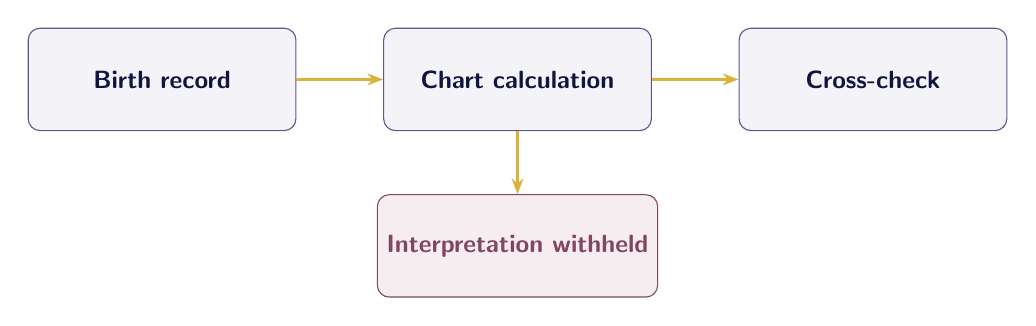
\begin{tikzpicture}[node distance=8mm and 11mm]
  \tikzset{
    stage/.style={rounded corners=1.5mm,draw=Purple,fill=Mist,minimum width=34mm,
      minimum height=13mm,align=center,font=\sffamily\small\bfseries,text=Navy},
    stop/.style={stage,draw=Burgundy,fill=PaleBurgundy,text=Burgundy},
    flow/.style={-{Stealth[length=2mm]},Gold,line width=.8pt}
  }
  \node[stage] (a) {Birth record};
  \node[stage,right=of a] (b) {Chart calculation};
  \node[stage,right=of b] (c) {Cross-check};
  \node[stop,below=of b] (d) {Interpretation withheld};
  \draw[flow] (a)--(b);
  \draw[flow] (b)--(c);
  \draw[flow] (b)--(d);
\end{tikzpicture}
\end{center}

\TwoCol{%
\begin{insightbox}
\BoxTitle{Required before personalization}
\begin{itemize}
  \item Client name and confirmed birth record
  \item Zodiac, Ayanamsa and house configuration
  \item Rashi chart and planetary degrees
  \item Nakshatras and verified Dasha schedule
\end{itemize}
\end{insightbox}
}{%
\begin{goldbox}
\BoxTitle{Quality-control rule}
If two data exports disagree, the report should pause at the calculation layer.
Elegant design cannot compensate for an unverified chart.
\end{goldbox}
}

\ReportPage{CLIENT RECORD}{Birth Information}
{The smallest error in time or place can change houses, divisional charts and timing.}

{\small
\rowcolors{2}{Mist}{white}
\begin{tabularx}{\linewidth}{>{\sffamily\bfseries\color{Navy}}p{43mm} X
  >{\sffamily\bfseries\color{Navy}}p{32mm} X}
\toprule
Client name & \ClientName & Report type & \ReportType\\
Date of birth & \DateOfBirth & Time of birth & \TimeOfBirth\\
Birthplace & \BirthPlace & Time zone & \TimeZone\\
Latitude / longitude & \Latitude{} / \Longitude & Source / confidence & \BirthDataSource{} / \BirthDataConfidence\\
Report date & \ReportDate & Privacy & \PrivacyStatus\\
\bottomrule
\end{tabularx}}

\vspace{5mm}
\begin{navybox}
\WhiteTitle{Birth-time confidence}
The final report should record whether the time came from an official record, family
memory, prior rectification or an estimate. If time confidence is low, conclusions
that depend heavily on houses, Navamsha or fine-grained Dasha timing should be softened.
\end{navybox}

\vspace{3mm}
\TwoCol{%
\begin{insightbox}
\BoxTitle{Client confirmation}
Before calculation, the client should confirm local time, daylight-saving treatment,
place spelling and whether the recorded time refers to the beginning or completion of
the birth event.
\end{insightbox}
}{%
\begin{goldbox}
\BoxTitle{Scope note}
\BirthDataScopeNote
\end{goldbox}
}

\ReportPage{CALCULATION BASIS}{Chart Configuration}
{A transparent report states the astronomical and interpretive configuration used.}

{\small
\rowcolors{2}{Mist}{white}
\begin{tabularx}{\linewidth}{>{\sffamily\bfseries\color{Navy}}p{46mm} X p{36mm}}
\toprule
Setting & Recorded value & Status\\
\midrule
Zodiac & \ZodiacSystem & \ZodiacSystemStatus\\
Ayanamsa & \Ayanamsa & \AyanamsaStatus\\
House system / chart convention & \HouseSystem & \HouseSystemStatus\\
Node convention (true / mean) & \NodeMode & \NodeModeStatus\\
Calculation version & \CalculationVersion & \CalculationVersionStatus\\
Vimshottari basis & \VimshottariBasis & \VimshottariBasisStatus\\
Transit reference date / place & \TransitReference & \TransitReferenceStatus\\
Divisional charts included & \DivisionalChartsIncluded & \DivisionalChartsStatus\\
\bottomrule
\end{tabularx}}

\vspace{4mm}
\begin{goldbox}
\BoxTitle{Preferred Astro Sushil configuration}
If the production chart export specifies the \textbf{Sidereal Zodiac} and
\textbf{Lahiri Ayanamsa}, those settings should be reproduced exactly. They are not
assumed by the template. \ChartConfigurationNote
\end{goldbox}

\begin{insightbox}
\BoxTitle{Why configuration matters}
A client should be able to understand why a sign, house, Nakshatra or Dasha date
appears in the report. Recording the calculation basis also makes future updates
consistent and auditable.
\end{insightbox}

\ReportPage{CHART VISUALIZATION}{North Indian Kundli}
{The production report places the verified Rashi chart beside a concise reading guide.}

\TwoCol{%
\begin{center}
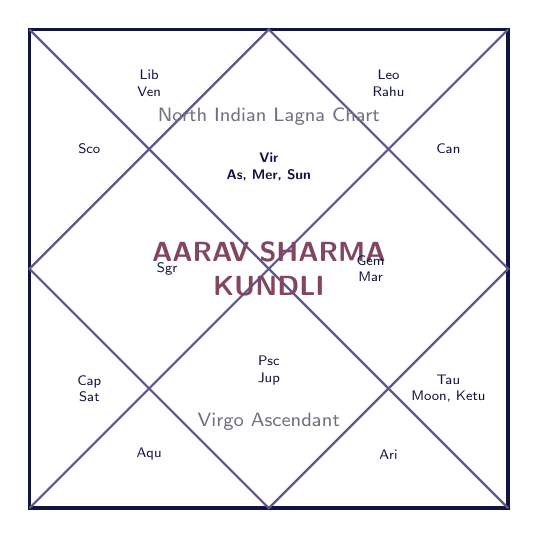
\begin{tikzpicture}[scale=.76]
  \draw[Navy,line width=1.3pt] (0,0) rectangle (8,8);
  \draw[Purple,line width=.8pt] (0,0)--(4,4)--(0,8);
  \draw[Purple,line width=.8pt] (8,0)--(4,4)--(8,8);
  \draw[Purple,line width=.8pt] (0,4)--(4,8)--(8,4)--(4,0)--cycle;
  \node[align=center,text=Burgundy,font=\sffamily\bfseries] at (4,4)
    {\KundliCenterLabel};
  \node[text=Muted,font=\sffamily\scriptsize] at (4,6.55) {\KundliUpperLabel};
  \node[text=Muted,font=\sffamily\scriptsize] at (4,1.45) {\KundliLowerLabel};
  \ifdefined\KundliHouseOne
    \node[align=center,text=Navy,font=\sffamily\tiny\bfseries] at (4,5.7) {\KundliHouseOne};
    \node[align=center,text=Navy,font=\sffamily\tiny] at (2,7.1) {\KundliHouseTwo};
    \node[align=center,text=Navy,font=\sffamily\tiny] at (1,6) {\KundliHouseThree};
    \node[align=center,text=Navy,font=\sffamily\tiny] at (2.3,4) {\KundliHouseFour};
    \node[align=center,text=Navy,font=\sffamily\tiny] at (1,2) {\KundliHouseFive};
    \node[align=center,text=Navy,font=\sffamily\tiny] at (2,0.9) {\KundliHouseSix};
    \node[align=center,text=Navy,font=\sffamily\tiny] at (4,2.3) {\KundliHouseSeven};
    \node[align=center,text=Navy,font=\sffamily\tiny] at (6,0.9) {\KundliHouseEight};
    \node[align=center,text=Navy,font=\sffamily\tiny] at (7,2) {\KundliHouseNine};
    \node[align=center,text=Navy,font=\sffamily\tiny] at (5.7,4) {\KundliHouseTen};
    \node[align=center,text=Navy,font=\sffamily\tiny] at (7,6) {\KundliHouseEleven};
    \node[align=center,text=Navy,font=\sffamily\tiny] at (6,7.1) {\KundliHouseTwelve};
  \fi
\end{tikzpicture}
\end{center}
}{%
\begin{unavailablebox}
\BoxTitle{Visualization status \hfill \ChartVisualizationStatus}
\ChartVisualizationNote
\end{unavailablebox}
\begin{insightbox}
\BoxTitle{Production standard}
The final chart should use the exact supplied longitudes, retain legible planet
labels, distinguish retrograde status where provided, and match the accompanying
placement table.
\end{insightbox}
}

\vspace{3mm}
\begin{navybox}
\WhiteTitle{Reading order}
Begin with the Ascendant and its lord, then the 10th house and 10th lord. Test the
career story against income (2nd), service and competition (6th), gains and networks
(11th), intelligence (5th), fortune and mentors (9th), and foreign or remote themes
(12th). Planetary condition and timing should refine—not replace—that synthesis.
\end{navybox}

\ReportPage{CHART REGISTER}{Planetary Placement Table}
{One verified table prevents interpretation from drifting away from the calculated chart.}

{\small
\rowcolors{2}{Mist}{white}
\begin{tabularx}{\linewidth}{>{\sffamily\bfseries\color{Navy}}l X X X X}
\toprule
Planet & Sign & House & Degree & Nakshatra / status\\
\midrule
\SunName & \SunSign & \SunHouse & \SunDegree & \SunNakshatra{} / \SunStatus\\
\MoonName & \MoonSign & \MoonHouse & \MoonDegree & \MoonNakshatra{} / \MoonStatus\\
\MarsName & \MarsSign & \MarsHouse & \MarsDegree & \MarsNakshatra{} / \MarsStatus\\
\MercuryName & \MercurySign & \MercuryHouse & \MercuryDegree & \MercuryNakshatra{} / \MercuryStatus\\
\JupiterName & \JupiterSign & \JupiterHouse & \JupiterDegree & \JupiterNakshatra{} / \JupiterStatus\\
\VenusName & \VenusSign & \VenusHouse & \VenusDegree & \VenusNakshatra{} / \VenusStatus\\
\SaturnName & \SaturnSign & \SaturnHouse & \SaturnDegree & \SaturnNakshatra{} / \SaturnStatus\\
\RahuName & \RahuSign & \RahuHouse & \RahuDegree & \RahuNakshatra{} / \RahuStatus\\
\KetuName & \KetuSign & \KetuHouse & \KetuDegree & \KetuNakshatra{} / \KetuStatus\\
\bottomrule
\end{tabularx}}

\vspace{4mm}
\TwoCol{%
\begin{insightbox}
\BoxTitle{Cross-checks}
The production editor should verify that sign, house, degree, Nakshatra, retrograde
status and combustion notes agree across the chart image, table and written analysis.
\end{insightbox}
}{%
\begin{goldbox}
\BoxTitle{Interpretive restraint}
Dignity is not a simple “good/bad” label. Functional role, ownership, placement,
aspects and the wider chart determine how a planet may express professionally.
\end{goldbox}
}

% --------------------------------------------------------------------------
% EXECUTIVE SUMMARY
% --------------------------------------------------------------------------
\ReportPage{EXECUTIVE SUMMARY I}{The Career Story at a Glance}
{The final three-page summary is designed to remain useful even if the client reads nothing else.}

\begin{unavailablebox}
\BoxTitle{Personalized career summary \hfill \ChartStatus}
\ExecutiveCareerSummary
\end{unavailablebox}

\begin{center}
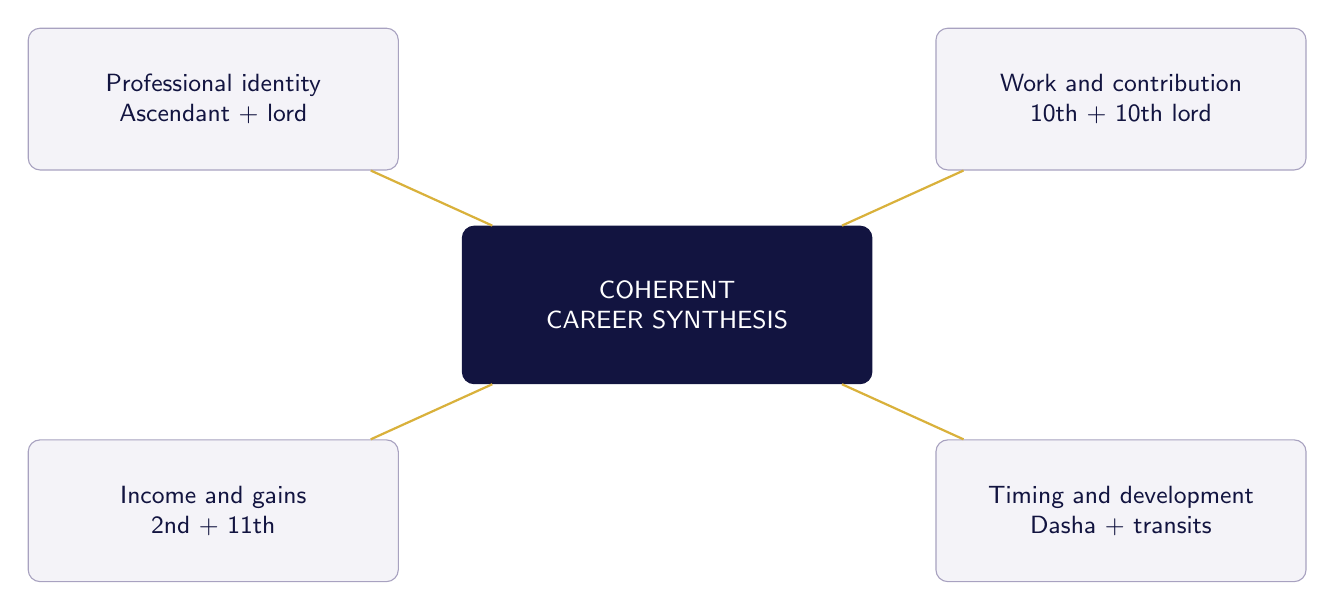
\begin{tikzpicture}[node distance=7mm and 8mm]
  \tikzset{
    card/.style={rounded corners=1.5mm,draw=Purple!55,fill=Mist,minimum width=47mm,
      minimum height=18mm,align=center,font=\sffamily\small,text=Navy},
    core/.style={card,fill=Navy,text=white,draw=Navy,minimum width=52mm,minimum height=20mm},
    link/.style={Gold,line width=.8pt}
  }
  \node[core] (c) {COHERENT\\CAREER SYNTHESIS};
  \node[card,above left=of c] (a) {Professional identity\\Ascendant + lord};
  \node[card,above right=of c] (b) {Work and contribution\\10th + 10th lord};
  \node[card,below left=of c] (d) {Income and gains\\2nd + 11th};
  \node[card,below right=of c] (e) {Timing and development\\Dasha + transits};
  \foreach \x in {a,b,d,e}{\draw[link] (\x)--(c);}
\end{tikzpicture}
\end{center}

\begin{navybox}
\WhiteTitle{Executive principle}
A premium consultation should not leave the client with disconnected observations.
It should explain the central professional pattern, where that pattern is most likely
to work well, what may complicate it, and which practical choices remain in the
client’s control.
\end{navybox}

\ReportPage{EXECUTIVE SUMMARY II}{Decision-Relevant Themes}
{The summary converts technical evidence into a short list of professional choices.}

\begin{unavailablebox}
\BoxTitle{Generated decision themes \hfill \ChartStatus}
\ExecutiveDecisionThemes
\end{unavailablebox}

\begin{tabularx}{\linewidth}{>{\sffamily\bfseries\color{Navy}}p{42mm} X p{38mm}}
\toprule
Decision area & Evidence required & Current status\\
\midrule
Career personality & Ascendant, lord, Moon, Sun, 10th & \ChartStatus\\
Top strengths & Repeated supported factors, dignity, Vargas & \ChartStatus\\
Top challenges & Afflictions, conflicts, Dasha activation & \ChartStatus\\
Leadership potential & Sun, Mars, Saturn, 10th, 11th & \ChartStatus\\
Entrepreneurship & 3rd, 7th, 10th, 11th, risk pattern & \ChartStatus\\
International potential & 9th, 12th, Rahu and timing & \ChartStatus\\
Major periods & Verified Vimshottari schedule / transits & \DashaStatus\\
\bottomrule
\end{tabularx}

\vspace{4mm}
\TwoCol{%
\begin{insightbox}
\BoxTitle{Best work environments}
The final summary should name environmental characteristics—such as autonomy,
structure, public visibility, research depth or cross-functional work—before naming
job titles. Environments often transfer across industries.
\end{insightbox}
}{%
\begin{goldbox}
\BoxTitle{Recommendation threshold}
A field should be called “strongly supported” only when multiple chart factors point
in the same direction and the relevant timing does not materially contradict them.
\end{goldbox}
}

\vspace{3mm}
{\displayfont\fontsize{15}{19}\selectfont\color{Navy}
Clarity comes from ranking evidence, not from listing every possible profession.}

\ReportPage{EXECUTIVE SUMMARY III}{Key Recommendations}
{A good recommendation is specific enough to act on and flexible enough to respect real life.}

\begin{insightbox}
\BoxTitle{Generated executive recommendations \hfill \ChartStatus}
\ExecutiveRecommendations
\end{insightbox}

\begin{navybox}
\WhiteTitle{Recommendations that can be made now}
\begin{enumerate}
  \item Obtain and verify the complete birth record and calculation export.
  \item Separate astrological reflection from factual career evidence: skills,
  experience, finances, market conditions and responsibilities.
  \item Use the final reading to compare a small number of real options rather than
  search for one “destined” profession.
  \item Convert each interpretation into a low-risk test: a project, conversation,
  course, portfolio piece, client pilot or role-shadowing exercise.
\end{enumerate}
\end{navybox}

\vspace{4mm}
\TwoCol{%
\begin{goldbox}
\BoxTitle{Leadership}
No level or style can be assigned yet. The production report will evaluate authority,
initiative, patience, accountability and network stewardship separately.
\end{goldbox}
\begin{insightbox}
\BoxTitle{Entrepreneurship}
The final reading will distinguish founder potential from the practical readiness to
take financial, operational and market risk.
\end{insightbox}
}{%
\begin{insightbox}
\BoxTitle{International work}
Foreign links can manifest as relocation, remote teams, multinational institutions,
export activity, cross-cultural work or learning—not relocation alone.
\end{insightbox}
\begin{goldbox}
\BoxTitle{Timing}
No major period can be named without verified Dasha dates. Any future production
version should print exact start and end dates and state the reference system.
\end{goldbox}
}

% --------------------------------------------------------------------------
% CAREER DNA AND CORE FACTORS
% --------------------------------------------------------------------------
\ReportPage{CAREER DNA}{Career DNA}
{Ten professional dimensions, summarized only after the underlying chart evidence has been weighed.}

\begin{unavailablebox}
\BoxTitle{Interpretive representation—not a scientific score \hfill \ChartStatus}
\CareerDNAAnalysis{} In the final report, any visual scale represents the
astrologer’s synthesis rather than a validated psychological measurement.
\end{unavailablebox}

{\small
\rowcolors{2}{Mist}{white}
\begin{tabularx}{\linewidth}{>{\sffamily\bfseries\color{Navy}}p{34mm} X p{41mm}}
\toprule
Dimension & Evidence typically reviewed & Status\\
\midrule
Leadership & Sun, Mars, Saturn, Ascendant, 10th/11th & \ChartStatus\\
Analysis & Mercury, Mars, 5th/6th/8th & \ChartStatus\\
Communication & Mercury, 2nd/3rd/5th/10th & \ChartStatus\\
Creativity & Venus, Moon, 5th, relevant links & \ChartStatus\\
Discipline & Saturn, 6th, 10th, repetition across chart & \ChartStatus\\
Risk-taking & Mars, Rahu, 3rd/5th/8th, stabilizers & \ChartStatus\\
Independence & Ascendant, 3rd, 10th lord, Sun/Rahu & \ChartStatus\\
Collaboration & Moon, Venus, Jupiter, 7th/11th & \ChartStatus\\
Persistence & Saturn, fixed signs, 6th/10th & \ChartStatus\\
Adaptability & Mercury, Moon, dual signs, Rahu & \ChartStatus\\
\bottomrule
\end{tabularx}}

\ReportPage{CORE PROFILE}{Your Professional Personality}
{Professional identity is the pattern of contribution, motivation and behavior that follows you across job titles.}

\begin{unavailablebox}
\BoxTitle{Generated career identity \hfill \ChartStatus}
\CareerIdentity
\end{unavailablebox}

\TwoCol{%
\begin{insightbox}
\BoxTitle{Identity layer}
The Ascendant and its lord describe how a person approaches life and initiates action.
The Sun adds questions of purpose, visibility and authority; the Moon describes
emotional rhythm and the conditions needed for sustained engagement.
\end{insightbox}
\begin{goldbox}
\BoxTitle{Work layer}
The 10th house, 10th lord and planets connected with them show how professional
responsibility may be carried and how contribution becomes visible.
\end{goldbox}
}{%
\begin{navybox}
\WhiteTitle{Synthesis questions}
\begin{itemize}
  \item Does the chart prefer depth, variety, structure or autonomy?
  \item Is recognition sought publicly or through mastery?
  \item Does pressure sharpen performance or fragment attention?
  \item Is authority expressed directly, relationally or technically?
\end{itemize}
\end{navybox}
}

\vspace{4mm}
\begin{unavailablebox}
\BoxTitle{Client interpretation \hfill \ChartStatus}
\ProfessionalPersonality
\end{unavailablebox}

\ReportPage{CORE PROFILE}{Your Natural Strengths}
{Strength is a repeatable capacity that becomes more useful when paired with context and practice.}

\begin{navybox}
\WhiteTitle{How strengths are identified}
Astro Sushil looks for repetition: a theme supported by the Ascendant, relevant house
lords, planetary condition and career houses carries more weight than an isolated
symbol. A strong planet may supply capacity; a connected house shows where the
capacity is likely to matter; timing can show when it becomes more prominent.
\end{navybox}

\vspace{3mm}
\TwoCol{%
\begin{insightbox}
\BoxTitle{Capacity}
Examples include analytical precision, persuasive communication, operational
discipline, strategic judgment, creative synthesis, endurance or relationship
building. No item is assigned without chart support.
\end{insightbox}
}{%
\begin{goldbox}
\BoxTitle{Context}
A capacity can express differently by environment. Communication may become teaching,
sales, writing, negotiation or product strategy; the rest of the chart helps narrow
the expression.
\end{goldbox}
}

\vspace{3mm}
\begin{unavailablebox}
\BoxTitle{Top strengths \hfill \ChartStatus}
\NaturalStrengths
\end{unavailablebox}

\ReportPage{CORE PROFILE}{Your Professional Challenges}
{A challenge is most useful when translated into a behavior that can be observed and managed.}

\TwoCol{%
\begin{unavailablebox}
\BoxTitle{What will be examined}
Conflicting house agendas, afflicted or weak significators, overemphasized planets,
unstable motivation, authority tension, perfectionism, risk concentration and
periods that activate difficult combinations.
\end{unavailablebox}
}{%
\begin{insightbox}
\BoxTitle{What will not be done}
The report will not label a person as doomed, unlucky, incapable or permanently
blocked. It will not turn Saturn, Rahu, Ketu or the 8th/12th houses into fear-based
predictions.
\end{insightbox}
}

\vspace{4mm}
\begin{navybox}
\WhiteTitle{From symbol to strategy}
Each final challenge should be written in four parts: the astrological pattern, the
possible workplace behavior, the situation that tends to trigger it, and one practical
countermeasure. This keeps the reading grounded and avoids fatalism.
\end{navybox}

\vspace{3mm}
\begin{goldbox}
\BoxTitle{Client interpretation \hfill \ChartStatus}
\ProfessionalChallenges{} Missing data is a report limitation, not a client trait.
\end{goldbox}

\ReportPage{ASCENDANT}{Ascendant and Professional Identity}
{The Ascendant anchors how the person meets opportunity, pressure and responsibility.}

\begin{unavailablebox}
\BoxTitle{Ascendant sign and degree \hfill \AscendantStatus}
Sign: \AscendantSign\quad Degree: \AscendantDegree\quad
Nakshatra: \AscendantNakshatra\quad Pada: \AscendantPada\par
\AscendantCareerInterpretation
\end{unavailablebox}

\TwoCol{%
\begin{insightbox}
\BoxTitle{Professional lens}
From an astrological perspective, the Ascendant can describe the style through which
talent is expressed: initiating, stabilizing, adapting, analyzing, relating,
protecting, competing or organizing. The rest of the chart determines the actual
career context.
\end{insightbox}
}{%
\begin{goldbox}
\BoxTitle{Career-axis relationship}
The final reading should compare the Ascendant with the 10th house. Harmony may make
professional roles feel identity-consistent; tension can indicate a meaningful gap
between personal style and public responsibility.
\end{goldbox}
}

\begin{navybox}
\WhiteTitle{Synthesis target}
The completed page should answer: “How do I naturally enter professional situations,
and what kind of public role asks me to grow beyond that default?”
\end{navybox}

\ReportPage{ASCENDANT}{Ascendant Lord Analysis}
{The Ascendant lord shows where personal agency is invested and how identity develops through experience.}

\begin{unavailablebox}
\BoxTitle{Lord, sign, house, degree and condition \hfill \AscendantLordStatus}
Lord: \AscendantLord\quad Sign: \AscendantLordSign\quad House: \AscendantLordHouse\quad
Degree: \AscendantLordDegree\par
Nakshatra: \AscendantLordNakshatra\quad Condition: \AscendantLordCondition\par
Relationships: \AscendantLordRelationships\par
\AscendantLordInterpretation
\end{unavailablebox}

\TwoCol{%
\begin{insightbox}
\BoxTitle{What the placement can clarify}
The house placement can show where effort and self-definition concentrate. Its links
with the 10th lord, 2nd, 6th or 11th houses can connect identity with contribution,
service, earnings and gains.
\end{insightbox}
}{%
\begin{goldbox}
\BoxTitle{Strength is contextual}
A well-supported lord may improve coherence and resilience, while pressure can show
development through effort or changing circumstances. Neither should be interpreted
without functional role and the whole chart.
\end{goldbox}
}

\begin{navybox}
\WhiteTitle{Practical output}
The final interpretation should convert the placement into a professional operating
principle—for example, how the client builds credibility, responds to uncertainty or
chooses between autonomy and institutional support.
\end{navybox}

\HousePage{The 10th House: Career and Karma}{HouseTen}
{The 10th house is the report’s central arena for vocation, responsibility, contribution and public standing.}
{The sign on the 10th, planets occupying it, influences upon it and the quality of its
lord describe the form and tone of professional responsibility. “Karma” here is used
in its traditional sense of action and duty, not as a promise of status.}
{Review the 10th sign and lord; occupants and aspects; the lord’s dignity, house,
Nakshatra and dispositor; links with the Ascendant and 2nd/6th/11th houses; relevant
Vargas and yogas; then confirm whether the active Dasha supports the same story.}
{The final page must unite these factors into one explanation of how the client tends
to build authority, what work is worth sustained effort, and where public contribution
is most credible. Isolated factor-by-factor commentary is not enough.}

\ReportPage{10TH HOUSE}{10th Lord Analysis}
{The 10th lord carries the agenda of career into the house and sign where it is placed.}

\begin{unavailablebox}
\BoxTitle{10th lord and placement \hfill \HouseTenStatus}
Lord: \HouseTenLord\quad Placement: \HouseTenLordPlacement\quad
Condition: \HouseTenCondition\quad Nakshatra links: \HouseTenNakshatraInfo
\end{unavailablebox}

\TwoCol{%
\begin{insightbox}
\BoxTitle{Placement logic}
The house occupied by the 10th lord often shows where professional effort, visibility
or responsibility becomes concentrated. Its sign can modify style; conjunctions and
aspects can add competing or complementary agendas.
\end{insightbox}
}{%
\begin{goldbox}
\BoxTitle{Critical relationships}
Particular attention goes to links with the Ascendant lord, wealth houses (2nd/11th),
service (6th), intelligence (5th), fortune (9th), partnership (7th) and foreign or
institutional settings (12th).
\end{goldbox}
}

\begin{navybox}
\WhiteTitle{Professional synthesis}
The final reading should distinguish \emph{what} the person contributes, \emph{where}
that contribution is likely to be valued, and \emph{how} authority is earned over time.
\end{navybox}

\HousePage{6th House: Employment and Competition}{HouseSix}
{The 6th house helps describe service, daily work, systems, competition, problem-solving and professional friction.}
{Traditionally, this house can show the ability to manage routine, obligations,
adversity, colleagues and competitive environments. It is especially relevant when
comparing structured employment with independent work.}
{Assess the sign, lord and occupants; links to the 10th and 11th; the condition of
Saturn and Mars; and whether the pattern supports sustainable service or produces
chronic conflict, overwork or scattered effort.}
{The final interpretation should explain the kind of problems the client is equipped
to solve, the level of structure that helps performance, and the work habits needed
to keep competition constructive.}

\HousePage{2nd House: Wealth and Earnings}{HouseTwo}
{The 2nd house adds earning capacity, accumulated resources, speech, values and financial continuity to the career story.}
{Career income is not judged from the 2nd house alone. Its lord, occupants and links
with the 10th and 11th can describe how knowledge, voice, family resources or stored
value connect with professional life.}
{Review stability versus volatility, the condition of wealth significators, links
with service or enterprise houses, and the active Dasha. Separate earning style from
actual financial advice.}
{The final page should clarify whether income is likely to be tied more strongly to
specialist knowledge, communication, management, assets, relationships or repeated
service—only when supported by the chart.}

\HousePage{11th House: Gains and Networks}{HouseEleven}
{The 11th house concerns gains, professional networks, audiences, alliances and the ability to scale results.}
{This house can show how opportunity travels through communities, institutions,
patrons, clients or large systems. It also helps distinguish personal competence from
the ability to convert competence into reach and reward.}
{Examine the 11th lord, occupants, relationship with the 2nd and 10th, Jupiter and
Saturn, and whether Rahu expands networks constructively or creates unstable
expectations.}
{The final synthesis should identify the quality of network that matters: senior
mentors, peer communities, public audience, enterprise clients, global teams or
long-term institutional relationships.}

\HousePage{5th House: Intelligence and Creativity}{HouseFive}
{The 5th house contributes strategic intelligence, authorship, creativity, judgment, learning style and calculated risk.}
{In career analysis, this house can describe how a person generates original ideas,
teaches, advises, designs, speculates or turns knowledge into a recognizable point of
view.}
{Assess the lord, occupants, Mercury, Jupiter and Venus; links with the 10th and 11th;
and whether creativity is disciplined enough to produce consistent professional
value.}
{The completed reading should distinguish creativity from artistic work. Strategy,
research design, product thinking, teaching and entrepreneurship can also be 5th-house
expressions when the wider chart supports them.}

\HousePage{9th House: Higher Learning and Fortune}{HouseNine}
{The 9th house adds higher learning, mentors, ethics, worldview, long-distance connection and fortunate openings.}
{Traditionally, the 9th can show how guidance, education, institutional legitimacy and
belief systems shape professional direction. “Fortune” should be interpreted as
context and opportunity, not guaranteed ease.}
{Review the lord, Jupiter, links with the 10th and Ascendant, education indicators,
foreign connections and whether Dasha activation makes learning, certification or
mentorship especially relevant.}
{The final synthesis should tell the client when expertise, ethical consistency,
credentialing or a strong mentor network may matter more than immediate visibility.}

\HousePage{12th House: Foreign, Remote and Institutional Work}{HouseTwelve}
{The 12th house may connect career with distant places, global systems, remote work, institutions, retreat or behind-the-scenes contribution.}
{A 12th-house emphasis does not automatically mean emigration or loss. It may manifest
through multinational teams, hospitals, universities, research labs, charities,
cross-border business, remote work or private specialist roles.}
{Assess the lord and occupants; links with the 9th, 10th and 11th; Rahu/Ketu; and
verified timing. Weigh practical relocation factors separately from symbolism.}
{The completed interpretation should name the likely form of “distance” or
institutional setting and explain whether it supports focus, service, specialization
or international reach.}

% --------------------------------------------------------------------------
% PLANETS
% --------------------------------------------------------------------------
\PlanetPage{\SunName}
{The Sun is traditionally associated with purpose, visibility, authority, confidence and the relationship with leadership.}
{Its sign, house and relationships can show how recognition is sought, how authority
is handled and where the person needs to act from a coherent center rather than from
approval-seeking.}
{Clear ownership, principled leadership, healthy visibility, willingness to decide and
the capacity to represent a team or institution.}
{Over-identification with title, sensitivity to recognition, conflict with authority
or reluctance to share credit—only if supported by the actual placement.}
{Check dignity, the house ruled, links with the 10th and Ascendant, Saturn contacts,
Nakshatra and the active Dasha.}
{Translate the Sun into a leadership practice: define the responsibility that should
be owned, the standard that should be represented and the ego-risk that should be managed.}

\PlanetPage{\MoonName}
{The Moon reflects emotional rhythm, responsiveness, public connection, adaptability and the conditions needed for sustained engagement.}
{In professional life, the Moon can indicate how atmosphere, people and changing
demands affect concentration and motivation. It may also relate to public-facing work
or care-oriented intelligence when connected with career factors.}
{Attunement to people, timing and context; relational judgment; adaptability; the
ability to notice needs that purely technical analysis may miss.}
{Mood-dependent productivity, porous boundaries, overreaction to feedback or frequent
direction changes—only where the chart confirms these tendencies.}
{Check phase and strength where available, sign/house, Nakshatra, aspects, lordship,
links with Mercury and the 10th, and Dasha activation.}
{Build a work rhythm that protects attention while preserving responsiveness. The
final report should name the environment that supports emotional steadiness.}

\PlanetPage{\MarsName}
{Mars is associated with initiative, courage, competition, engineering action, conflict and the ability to execute under pressure.}
{Its placement can describe how quickly a person moves from intention to action, what
kind of challenge mobilizes effort, and whether professional force becomes precision
or friction.}
{Decisiveness, technical problem-solving, stamina, constructive competition, crisis
response and the willingness to confront obstacles directly.}
{Impatience, avoidable conflict, rushed decisions, burnout or treating collaboration
as a contest—only if repeated elsewhere in the chart.}
{Review sign/house, dignity, lordship, aspects to career houses, Saturn relationship,
Nakshatra, combustion and current periods.}
{Channel Mars into a defined arena with clear rules, measurable outcomes and recovery
time. Energy without a target should not be mistaken for career direction.}

\PlanetPage{\MercuryName}
{Mercury governs analysis, language, trade, systems, learning, negotiation and the movement of information.}
{Career relevance may appear through writing, data, technology, finance, consulting,
product work, sales, teaching or coordination, depending on the houses and planets
Mercury connects.}
{Curiosity, pattern recognition, clear explanation, commercial awareness, iteration
and the ability to translate between technical and non-technical groups.}
{Overanalysis, fragmented attention, cleverness without depth, nervous overwork or
constant switching—only where the placement supports it.}
{Check sign, house, dignity, combustion, retrogression if supplied, conjunctions,
lordship, 2nd/5th/10th links and Dasha activation.}
{The final reading should name the medium through which Mercury creates value:
analysis, communication, transactions, design of systems or synthesis of knowledge.}

\PlanetPage{\JupiterName}
{Jupiter is associated with judgment, expansion, teaching, counsel, ethics, institutions and the ability to see a larger framework.}
{In a career report, Jupiter can show where experience becomes guidance, where
credibility grows through knowledge, and how opportunity is related to mentors,
education or institutional trust.}
{Strategic perspective, generosity, teaching, sound counsel, confidence-building and
the capacity to connect work with meaning.}
{Overextension, abstract optimism, credential dependence, moral certainty or promises
larger than execution—only if the chart indicates these risks.}
{Assess sign/house, functional role, dignity, links with 5th/9th/10th/11th, aspects,
Nakshatra and relevant Dasha periods.}
{Convert Jupiter into a practice of judgment: deepen expertise, teach what has been
tested, and distinguish genuine scale from expansion for its own sake.}

\PlanetPage{\VenusName}
{Venus relates to value, aesthetics, agreement, relationships, refinement, comfort and the ability to create attractive exchange.}
{Professionally, Venus may support design, diplomacy, client experience, negotiation,
branding, finance, hospitality or any role where taste and relationship quality
create measurable value.}
{Refinement, tact, collaborative intelligence, proportion, audience sensitivity and
the ability to make an offering more desirable or humane.}
{Conflict avoidance, comfort-seeking, blurred commercial boundaries or prioritizing
appearance over substance—only when supported by placement.}
{Review sign/house, dignity, lordship, connections with Mercury and career houses,
combustion, Nakshatra and timing.}
{The final report should identify what Venus is helping the client value, improve or
negotiate—and the standard needed to keep refinement commercially grounded.}

\PlanetPage{\SaturnName}
{Saturn is central to career analysis through responsibility, structure, endurance, limits, craft and long-term authority.}
{Saturn often describes where competence is built slowly and where consequences make
standards unavoidable. Its role should be read with maturity, not reduced to delay or
punishment.}
{Patience, process discipline, realism, operational reliability, accountability and
the ability to build durable expertise or institutions.}
{Fear of failure, excessive caution, rigidity, overwork, isolation or staying too long
in unrewarding structures—only if chart context supports it.}
{Check sign/house, dignity, lordship, links with the Ascendant and 10th, aspects to the
Sun/Moon/Mars, Nakshatra and active Dasha.}
{Define the long game: which responsibility is worth carrying, which system needs
improvement, and which limit should be respected rather than fought.}

\PlanetPage{\RahuName}
{Rahu is traditionally associated with appetite, amplification, novelty, boundary-crossing, ambition and unfamiliar environments.}
{In career matters, Rahu can correlate with technology, unconventional routes, foreign
networks, scale, visibility or restless ambition, depending entirely on placement and
dispositor support.}
{Bold experimentation, comfort with ambiguity, cross-cultural reach, rapid learning
and the willingness to enter emerging or non-traditional fields.}
{Obsession, inflated expectations, unstable alliances, status hunger or mistaking
novelty for value—only where the full chart confirms the pattern.}
{Review sign/house, dispositor, conjunctions, aspects, 10th/11th/12th connections,
Nakshatra and exact Dasha dates.}
{Use Rahu as a controlled experiment: define success criteria, ethical boundaries and
a review point before committing identity or capital to an amplified opportunity.}

\PlanetPage{\KetuName}
{Ketu is traditionally linked with detachment, concentration, discontinuity, inward mastery and reduced interest in conventional validation.}
{Professionally, Ketu may support specialist depth, research, diagnosis, spiritual or
technical concentration, or periodic disengagement from roles that feel superficial.}
{Independence from fashion, sharp pattern recognition, minimalism, specialist focus
and the ability to release methods that no longer serve the work.}
{Withdrawal, under-communication, abrupt disengagement, difficulty valuing ordinary
success or expertise that remains inaccessible to others—only if supported.}
{Assess sign/house, dispositor, conjunctions, 6th/8th/10th/12th links, Nakshatra and
timing; always read Ketu with Rahu as an axis.}
{Pair depth with translation. The final report should show how specialized insight can
be communicated, applied and integrated into a sustainable professional role.}

% --------------------------------------------------------------------------
% SYNTHESIS MATRICES
% --------------------------------------------------------------------------
\ReportPage{PLANETARY SYNTHESIS}{Planetary Strengths and Challenges}
{A planet becomes career-significant through condition, ownership, connection and timing—not by reputation alone.}

\begin{center}
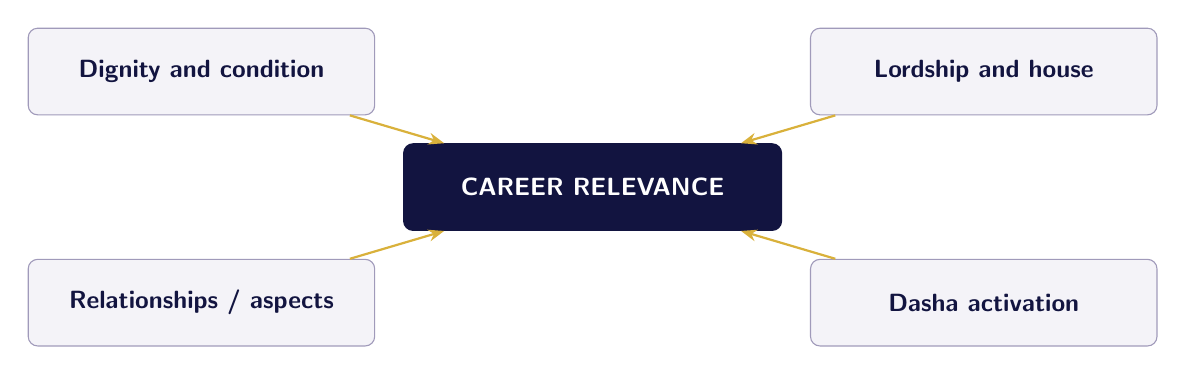
\begin{tikzpicture}[node distance=5mm]
  \tikzset{
    n/.style={draw=Purple!60,fill=Mist,rounded corners=1.2mm,minimum width=44mm,
      minimum height=11mm,align=center,font=\sffamily\small\bfseries,text=Navy},
    c/.style={n,fill=Navy,text=white,draw=Navy,minimum width=48mm},
    a/.style={-{Stealth[length=2mm]},Gold,line width=.8pt}
  }
  \node[c] (core) {CAREER RELEVANCE};
  \node[n,above left=of core] (d) {Dignity and condition};
  \node[n,above right=of core] (l) {Lordship and house};
  \node[n,below left=of core] (r) {Relationships / aspects};
  \node[n,below right=of core] (t) {Dasha activation};
  \foreach \x in {d,l,r,t}{\draw[a] (\x)--(core);}
\end{tikzpicture}
\end{center}

\TwoCol{%
\begin{insightbox}
\BoxTitle{Strength}
Strength can mean access, stability, visibility or the capacity to deliver a planet’s
agenda. It does not automatically mean that every result associated with that planet
will feel pleasant.
\end{insightbox}
}{%
\begin{goldbox}
\BoxTitle{Challenge}
A pressured planet may indicate effort, complexity, developmental work or uneven
expression. It should not be turned into a fixed negative identity.
\end{goldbox}
}

\begin{unavailablebox}
\BoxTitle{Client ranking \hfill \ChartStatus}
\PlanetarySynthesis
\end{unavailablebox}

\ReportPage{YOGAS}{Career-Significant Yogas}
{Yogas should be verified precisely, qualified by strength and integrated with the whole chart.}

\begin{unavailablebox}
\BoxTitle{Career-significant Yoga analysis \hfill \ChartStatus}
\YogaAnalysis
\end{unavailablebox}

\TwoCol{%
\begin{insightbox}
\BoxTitle{Verification protocol}
\begin{enumerate}
  \item State the exact rule used.
  \item Identify the planets and houses involved.
  \item Confirm sign, house and relationship.
  \item Qualify condition, functional role and activation.
  \item Explain the career relevance in plain language.
\end{enumerate}
\end{insightbox}
}{%
\begin{goldbox}
\BoxTitle{Interpretive caution}
A named Yoga is not a guarantee of status or wealth. The production report should
avoid ceremonial lists and focus only on combinations that materially change the
career synthesis.
\end{goldbox}
}

\begin{navybox}
\WhiteTitle{Editorial standard}
Every Yoga mentioned in the final document should be traceable to the placement table
and should add information not already conveyed more clearly by the house and planet
analysis.
\end{navybox}

\ReportPage{MATRIX}{Professional Strengths Matrix}
{A one-page evidence map makes the final ranking transparent and easy to revisit.}

{\small
\rowcolors{2}{Mist}{white}
\begin{tabularx}{\linewidth}{>{\sffamily\bfseries\color{Navy}}p{31mm} X X p{38mm}}
\toprule
Theme & Primary evidence & Corroborating evidence & Status\\
\midrule
Leadership & Sun / 10th / Ascendant & Mars, Saturn, 11th & \StrengthsMatrixStatus\\
Analysis & Mercury / 5th / 6th & Mars, 8th, Vargas & \StrengthsMatrixStatus\\
Communication & Mercury / 2nd / 3rd & 5th, 10th, Venus & \StrengthsMatrixStatus\\
Creativity & Venus / Moon / 5th & Mercury, 3rd, 10th & \StrengthsMatrixStatus\\
Execution & Mars / Saturn / 6th & 10th, fixed support & \StrengthsMatrixStatus\\
Strategy & Jupiter / Mercury / 5th & 9th, 10th, Saturn & \StrengthsMatrixStatus\\
Networks & 11th / Jupiter & Venus, Rahu, 7th & \StrengthsMatrixStatus\\
Global reach & 9th / 12th / Rahu & 10th, Dasha, transits & \StrengthsMatrixStatus\\
\bottomrule
\end{tabularx}}

\vspace{4mm}
\begin{goldbox}
\BoxTitle{How the final matrix should read}
Each strength will be ranked only after the astrologer records supporting and
contradictory factors. The matrix is a visual index of interpretation, not a
statistical test.
\end{goldbox}

\ReportPage{MATRIX}{Career Challenge Matrix}
{The goal is to identify manageable pressure patterns, not to assign permanent flaws.}

{\small
\rowcolors{2}{Mist}{white}
\begin{tabularx}{\linewidth}{>{\sffamily\bfseries\color{Navy}}p{31mm} X X p{38mm}}
\toprule
Possible pattern & Evidence needed & Practical counterweight & Status\\
\midrule
Overextension & Jupiter/Rahu + weak limits & Scope, sequencing, review gates & \ChallengeMatrixStatus\\
Impatience & Mars pressure / unstable links & Decision pause, clear escalation & \ChallengeMatrixStatus\\
Rigidity & Saturn/fixed overemphasis & Experiments, feedback cadence & \ChallengeMatrixStatus\\
Fragmentation & Mercury/Rahu volatility & Fewer priorities, deep-work blocks & \ChallengeMatrixStatus\\
Recognition tension & Sun/10th conflict & Role clarity, ownership language & \ChallengeMatrixStatus\\
Boundary strain & Moon/Venus/12th links & Availability norms, recovery & \ChallengeMatrixStatus\\
Withdrawal & Ketu/Saturn pressure & Communication rituals, visible work & \ChallengeMatrixStatus\\
\bottomrule
\end{tabularx}}

\vspace{4mm}
\begin{navybox}
\WhiteTitle{Use in consultation}
The astrologer should ask whether the proposed pattern is visible in the client’s
actual experience. When lived evidence contradicts the symbolic hypothesis, the
interpretation should be revised rather than defended.
\end{navybox}

% --------------------------------------------------------------------------
% WORK MODES AND POTENTIAL
% --------------------------------------------------------------------------
\ReportPage{WORK MODE}{Employment vs Entrepreneurship}
{The useful question is not “job or business?” but “which risk, structure and responsibility profile fits now?”}

{\small
\begin{tabularx}{\linewidth}{>{\sffamily\bfseries\color{Navy}}p{28mm} X X}
\toprule
Mode & Potential advantages & Evidence to assess\\
\midrule
Employment & Structure, team resources, stable learning, institutional reach &
6th/10th, Saturn, Sun, gains and timing\\
Entrepreneurship & Autonomy, ownership, upside, direct market feedback &
3rd/5th/7th/10th/11th, Mars, Mercury, Rahu\\
Freelancing & Flexible specialization, portfolio variety, controlled independence &
3rd/6th/7th, Mercury, Saturn, income stability\\
Consulting & Expertise, diagnosis, communication, relationship leverage &
Mercury/Jupiter, 5th/7th/10th/11th\\
Independent practice & Authority through mastery and trust &
Ascendant/10th, specialist houses, client indicators\\
\bottomrule
\end{tabularx}}

\vspace{3mm}
\begin{unavailablebox}
\BoxTitle{Client recommendation \hfill \ChartStatus}
\EmploymentEntrepreneurshipAnalysis\par
The final report should separate \textbf{temperamental fit} from
\textbf{readiness}: savings, market access, operating skill, dependents and risk
tolerance remain practical questions.
\end{unavailablebox}

\ReportPage{LEADERSHIP}{Leadership Potential}
{Leadership is examined as a set of behaviors: direction, judgment, accountability, influence and stewardship.}

\TwoCol{%
\begin{insightbox}
\BoxTitle{Astrological evidence}
Sun for authority and coherent purpose; Mars for initiative; Saturn for responsibility
and systems; Ascendant for style; 10th for public role; 11th for groups and scale;
relevant yogas and timing for activation.
\end{insightbox}
\begin{goldbox}
\BoxTitle{Leadership styles}
The final report may distinguish directive, expert, facilitative, operational,
visionary or relational leadership. A client may show more than one style across
different stages.
\end{goldbox}
}{%
\begin{navybox}
\WhiteTitle{Questions to answer}
\begin{itemize}
  \item How are decisions made under pressure?
  \item Is authority claimed, earned slowly or delegated?
  \item Does the person lead people, systems, ideas or clients?
  \item What weakness appears when responsibility expands?
  \item How may leadership mature over time?
\end{itemize}
\end{navybox}
}

\vspace{3mm}
\begin{unavailablebox}
\BoxTitle{Leadership conclusion \hfill \ChartStatus}
\LeadershipAnalysis
\end{unavailablebox}

\ReportPage{APTITUDE}{Technical and Analytical Potential}
{Technical potential combines problem selection, reasoning style, precision, persistence and the ability to ship reliable work.}

\begin{navybox}
\WhiteTitle{Evidence model}
Mercury may support symbolic reasoning and systems; Mars can add engineering action
and decisive troubleshooting; Saturn can supply rigor and repeatability; the 5th, 6th
and 8th houses may contribute intelligence, applied problem-solving and research
depth. Career links determine whether these capacities become vocational.
\end{navybox}

\vspace{3mm}
\TwoCol{%
\begin{insightbox}
\BoxTitle{Possible expressions}
Software, data, engineering, operations research, audit, quantitative work,
diagnostics, quality systems, cybersecurity or technical product roles—only if
supported by actual chart factors and lived skill.
\end{insightbox}
}{%
\begin{goldbox}
\BoxTitle{Potential challenges}
Analysis can become overengineering, isolation or slow decisions. Strong execution
without communication can limit influence. The final report should identify the
balancing capacity.
\end{goldbox}
}

\begin{unavailablebox}
\BoxTitle{Client aptitude conclusion \hfill \ChartStatus}
\TechnicalAnalyticalAptitude
\end{unavailablebox}

\ReportPage{APTITUDE}{Creative, Communication and Business Potential}
{Creative work becomes professionally durable when imagination, audience understanding and execution reinforce one another.}

\TwoCol{%
\begin{insightbox}
\BoxTitle{Creative evidence}
Venus, Moon, Mercury and the 5th house can contribute aesthetics, narrative,
imagination and authorship. Connections with the 10th and 11th help show whether
creative expression becomes public work or scalable value.
\end{insightbox}
\begin{goldbox}
\BoxTitle{Communication evidence}
Mercury, the 2nd and 3rd houses, Jupiter and career links can support writing,
teaching, negotiation, marketing, sales or translation between disciplines.
\end{goldbox}
}{%
\begin{navybox}
\WhiteTitle{Business expression}
Business potential requires more than persuasive ability. The final assessment also
reviews judgment, relationship management, risk, operational discipline, income
continuity and the capacity to learn from a market.
\end{navybox}
}

\vspace{3mm}
\begin{unavailablebox}
\BoxTitle{Client conclusion \hfill \ChartStatus}
\CreativeCommunicationBusinessAptitude
\end{unavailablebox}

\ReportPage{APTITUDE}{Research and Specialized Knowledge}
{Specialization grows where curiosity can tolerate uncertainty and discipline can sustain depth.}

\begin{center}
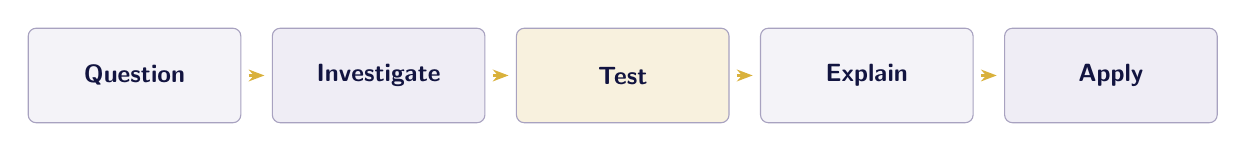
\begin{tikzpicture}
  \foreach \x/\label/\col in {0/Question/Mist,3.1/Investigate/PalePurple,6.2/Test/PaleGold,9.3/Explain/Mist,12.4/Apply/PalePurple}{
    \node[draw=Purple!55,fill=\col,rounded corners=1mm,minimum width=27mm,
      minimum height=12mm,font=\sffamily\small\bfseries,text=Navy] at (\x,0) {\label};
  }
  \foreach \x in {1.45,4.55,7.65,10.75}
    \draw[-{Stealth[length=2mm]},Gold,line width=.8pt] (\x,0)--++(.2,0);
\end{tikzpicture}
\end{center}

\TwoCol{%
\begin{insightbox}
\BoxTitle{Chart factors}
Mercury and Jupiter for knowledge, Saturn for sustained method, Mars for testing,
Ketu for concentration, Rahu for new domains, and the 5th/8th/9th/12th houses for
different forms of inquiry.
\end{insightbox}
}{%
\begin{goldbox}
\BoxTitle{Professional test}
Depth must connect to a user, decision, institution, publication, product or problem.
The final report should explain how specialist knowledge reaches the 10th and 11th
houses of contribution and gain.
\end{goldbox}
}

\begin{unavailablebox}
\BoxTitle{Research potential \hfill \ChartStatus}
\ResearchPotential
\end{unavailablebox}

\ReportPage{SECTOR FIT}{Government, Corporate and Private-Sector Tendencies}
{Institutional fit depends on the kind of authority, scale, structure and public responsibility a chart can sustain.}

{\small
\begin{tabularx}{\linewidth}{>{\sffamily\bfseries\color{Navy}}p{33mm} X X}
\toprule
Environment & Typical demands & Factors to review\\
\midrule
Government / public service & Procedure, accountability, continuity, public mandate &
Sun, Saturn, 6th/9th/10th, service links\\
Large corporate & Scale, specialization, hierarchy, cross-functional influence &
Saturn, Mercury, 10th/11th, network capacity\\
Private / growth company & Ambiguity, speed, commercial judgment, ownership &
Mars, Mercury, Rahu, 3rd/7th/10th/11th\\
Professional practice & Expertise, trust, reputation, client continuity &
Jupiter, Mercury, 7th/9th/10th, income links\\
Mission-led institution & Values, service, resource constraints, stakeholder balance &
Jupiter, Moon, 6th/9th/12th, Saturn\\
\bottomrule
\end{tabularx}}

\vspace{3mm}
\begin{unavailablebox}
\BoxTitle{Sector preference \hfill \ChartStatus}
\SectorFit\par
The final recommendation should identify the \emph{institutional conditions} that fit
before naming a sector.
\end{unavailablebox}

\ReportPage{GLOBAL CAREER}{International and Foreign Career Potential}
{Foreign potential is broader than relocation: it can mean clients, teams, institutions, trade, learning or digital reach across borders.}

\TwoCol{%
\begin{insightbox}
\BoxTitle{Evidence reviewed}
9th and 12th houses and their lords; Rahu and its dispositor; connections with the
Ascendant and 10th; 7th/11th for external markets and networks; Dasha and transit
periods for timing.
\end{insightbox}
}{%
\begin{goldbox}
\BoxTitle{Forms of expression}
Relocation, study abroad, multinational employment, cross-border consulting, export,
remote teams, research institutions, immigration-linked work or culturally hybrid
roles.
\end{goldbox}
}

\begin{navybox}
\WhiteTitle{Decision standard}
Astrological symbolism should be combined with visa rules, finances, language,
family responsibilities, labor-market conditions and the quality of the actual
opportunity. A 12th-house theme is not a travel instruction.
\end{navybox}

\begin{unavailablebox}
\BoxTitle{Client potential and timing \hfill \ChartStatus}
\InternationalCareer
\end{unavailablebox}

\ReportPage{ENVIRONMENT}{Suitable Work Environments}
{A strong environment supports the client’s way of thinking, recovering, collaborating and taking responsibility.}

\begin{unavailablebox}
\BoxTitle{Client work-environment synthesis \hfill \ChartStatus}
\WorkEnvironment
\end{unavailablebox}

{\small
\rowcolors{2}{Mist}{white}
\begin{tabularx}{\linewidth}{>{\sffamily\bfseries\color{Navy}}p{34mm} X p{40mm}}
\toprule
Environment dimension & Questions for the final reading & Status\\
\midrule
Structure & Clear process or flexible method? & \ChartStatus\\
Pace & Deliberate depth or rapid iteration? & \ChartStatus\\
Visibility & Public ownership or behind-the-scenes mastery? & \ChartStatus\\
Autonomy & Independent decisions or collaborative alignment? & \ChartStatus\\
Problem type & People, systems, ideas, assets or crises? & \ChartStatus\\
Scale & Small specialist team or large institution? & \ChartStatus\\
Feedback & Immediate market signal or long research cycle? & \ChartStatus\\
Geography & Local, remote, mobile or cross-border? & \ChartStatus\\
\bottomrule
\end{tabularx}}

\vspace{4mm}
\begin{goldbox}
\BoxTitle{Practical use}
When comparing two roles, score the factual environment first. The astrology can then
be used as a reflective lens on fit, but the actual manager, mandate, resources and
career path remain decisive.
\end{goldbox}

% --------------------------------------------------------------------------
% CAREER FIELDS, MONEY AND PEOPLE
% --------------------------------------------------------------------------
\ReportPage{CAREER FIELDS}{Career Fields and Industry Analysis}
{Fields are recommended only when several chart factors converge on a consistent type of work.}

\begin{unavailablebox}
\BoxTitle{Generated career-field analysis \hfill \ChartStatus}
\CareerFieldsAnalysis
\end{unavailablebox}

\begin{navybox}
\WhiteTitle{Ranking method}
For each field, the production report should cite: (1) the work function indicated,
(2) the houses and planets supporting it, (3) the role level or work mode that fits,
(4) the principal challenge, and (5) whether current timing favors exploration,
preparation, consolidation or expansion.
\end{navybox}

\vspace{3mm}
{\small
\begin{tabularx}{\linewidth}{>{\sffamily\bfseries\color{Navy}}p{36mm} X X}
\toprule
Field family & Example functions & Required evidence\\
\midrule
Technology / engineering & Build, automate, secure, optimize & Mercury/Mars/Saturn + career links\\
Research / science / medicine & Investigate, diagnose, validate & 5th/6th/8th/9th + relevant planets\\
Finance / management & Allocate, govern, plan, scale & 2nd/10th/11th + judgment factors\\
Education / consulting / law & Explain, advise, interpret, advocate & Mercury/Jupiter/Sun + 5th/9th/10th\\
Marketing / media / design & Position, narrate, attract, engage & Mercury/Venus/Moon + 3rd/5th/11th\\
Operations / manufacturing & Standardize, deliver, improve & Mars/Saturn + 6th/10th/11th\\
\bottomrule
\end{tabularx}}

\ReportPage{CAREER FIELDS}{Top Career Directions and Caution Areas}
{A premium report narrows choices; it does not present a catalogue of every profession.}

\begin{unavailablebox}
\BoxTitle{Ranked career directions \hfill \ChartStatus}
\TopCareerDirections\par
\textbf{Caution areas:} \CareerDirectionsCaution
\end{unavailablebox}

\TwoCol{%
\begin{insightbox}
\BoxTitle{For each recommended direction}
\begin{itemize}
  \item Why it is astrologically supported
  \item Which role family fits best
  \item What advantage the client may bring
  \item What difficulty needs management
  \item What low-risk experiment can test fit
\end{itemize}
\end{insightbox}
}{%
\begin{goldbox}
\BoxTitle{For each caution area}
The report should explain the mismatch precisely: pace, exposure, authority,
repetition, financial risk, emotional load, ethical tension or skill gap. “Not in your
destiny” is neither precise nor responsible.
\end{goldbox}
}

\begin{navybox}
\WhiteTitle{Production target}
Rank three primary directions, two adjacent alternatives and no more than three
caution areas. Fewer, well-supported options create more value than a long list.
\end{navybox}

\ReportPage{MONEY}{Money and Income Patterns}
{The chart may describe earning themes; it does not replace financial planning or guarantee income.}

\TwoCol{%
\begin{insightbox}
\BoxTitle{What is assessed}
The 2nd for accumulation and value; 6th for service and recurring work; 10th for
professional contribution; 11th for gains and scale; 5th for calculated risk; 8th for
shared resources; relevant lords, significators and timing.
\end{insightbox}
}{%
\begin{goldbox}
\BoxTitle{What is separated}
Earning capacity, cash-flow stability, appetite for risk, spending behavior and
wealth accumulation are different questions. A career report should not collapse
them into one “money Yoga.”
\end{goldbox}
}

\begin{navybox}
\WhiteTitle{Practical interpretation}
The final report should identify whether income is better supported by specialization,
volume, relationships, institutional progression, ownership, assets or multiple
channels—then compare that interpretation with the client’s actual financial position.
\end{navybox}

\begin{unavailablebox}
\BoxTitle{Client income pattern \hfill \ChartStatus}
\MoneyIncomePattern
\end{unavailablebox}

\ReportPage{RELATIONSHIPS}{Professional Relationships and Networking}
{Career growth often depends on the quality of trust, reciprocity and information moving through a network.}

\TwoCol{%
\begin{insightbox}
\BoxTitle{Relationship factors}
Moon and Venus can contribute relational sensitivity; Mercury communication; Jupiter
mentorship; Saturn commitment; the 7th partnership; the 11th groups and gains; the
2nd speech and values.
\end{insightbox}
}{%
\begin{goldbox}
\BoxTitle{Network quality}
The final reading should distinguish broad reach from dependable alliances. Rahu may
amplify access; Saturn may favor slower trust; Jupiter may emphasize patrons or
teachers. Placement decides the expression.
\end{goldbox}
}

\begin{navybox}
\WhiteTitle{Practical framework}
Map five relationship categories: manager/sponsor, mentor, peer circle, collaborator,
and client/audience. For each, define the value exchanged and the cadence required to
maintain trust.
\end{navybox}

\begin{unavailablebox}
\BoxTitle{Client relationship pattern \hfill \ChartStatus}
\RelationshipsNetworking
\end{unavailablebox}

\ReportPage{TEAMS}{Leadership and Team Dynamics}
{Team fit depends on how authority, conflict, communication, care and accountability are balanced.}

{\small
\begin{tabularx}{\linewidth}{>{\sffamily\bfseries\color{Navy}}p{32mm} X X}
\toprule
Dynamic & Astrological lens & Practical observation\\
\midrule
Decision rights & Sun, Mars, 10th & Who decides, and after what input?\\
Standards & Saturn, 6th, 10th & How is quality defined and enforced?\\
Communication & Mercury, 2nd/3rd & What information is shared, when and how?\\
Belonging & Moon, Venus, 11th & What builds psychological safety and trust?\\
Conflict & Mars, Saturn, 6th/7th & How are disagreement and escalation handled?\\
Learning & Jupiter, 5th/9th & How does the team improve judgment?\\
\bottomrule
\end{tabularx}}

\vspace{4mm}
\begin{goldbox}
\BoxTitle{Development over time}
Leadership can mature as a person learns to combine decisive action with proportionate
process, and personal standards with explicit communication. Dasha periods may
describe which part of that developmental task is emphasized.
\end{goldbox}

\begin{unavailablebox}
\BoxTitle{Client team profile \hfill \ChartStatus}
\TeamDynamics
\end{unavailablebox}

\ReportPage{SUSTAINABILITY}{Work–Life Balance}
{Sustainable contribution requires a rhythm that protects health, attention, relationships and meaning.}

\TwoCol{%
\begin{insightbox}
\BoxTitle{Astrological reflection}
Moon can describe emotional rhythm; Saturn limits and duty; Mars expenditure of
energy; the 6th routines; 12th rest and withdrawal; 4th inner stability; 10th public
responsibility. The whole pattern matters.
\end{insightbox}
}{%
\begin{goldbox}
\BoxTitle{Practical evidence}
Sleep, caregiving, commute, workload, health, financial pressure, manager quality and
schedule control are more direct measures of sustainability and must remain central.
\end{goldbox}
}

\begin{navybox}
\WhiteTitle{Balance is not equal time}
The final recommendation should identify recovery needs, boundary risks and the type
of intensity that is sustainable. A demanding period may call for a narrower scope,
better support or explicit recovery—not a dramatic prediction.
\end{navybox}

\begin{unavailablebox}
\BoxTitle{Client sustainability pattern \hfill \ChartStatus}
\SustainabilityAnalysis
\end{unavailablebox}

\ReportPage{OBSTACLES}{Career Obstacles}
{An obstacle becomes actionable when its source, trigger, behavior and countermeasure are distinguished.}

\begin{center}
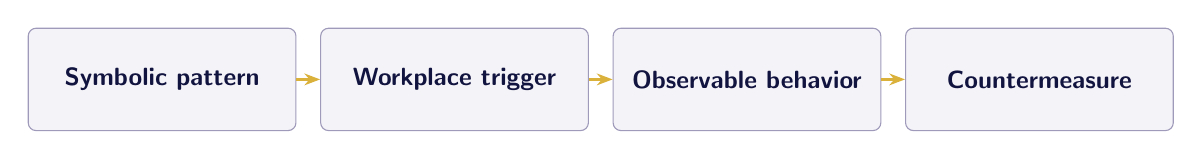
\begin{tikzpicture}[node distance=3mm]
  \tikzset{b/.style={draw=Purple!60,fill=Mist,rounded corners=1mm,minimum width=34mm,
    minimum height=13mm,align=center,font=\sffamily\small\bfseries,text=Navy},
    a/.style={-{Stealth[length=2mm]},Gold,line width=.8pt}}
  \node[b] (a) {Symbolic pattern};
  \node[b,right=of a] (b) {Workplace trigger};
  \node[b,right=of b] (c) {Observable behavior};
  \node[b,right=of c] (d) {Countermeasure};
  \draw[a] (a)--(b);\draw[a] (b)--(c);\draw[a] (c)--(d);
\end{tikzpicture}
\end{center}

\TwoCol{%
\begin{insightbox}
\BoxTitle{Internal obstacles}
Examples may include hesitation, impatience, perfectionism, conflict avoidance,
fragmented attention, status sensitivity or difficulty sustaining routine. None is
assigned without evidence.
\end{insightbox}
}{%
\begin{goldbox}
\BoxTitle{External obstacles}
Market conditions, discrimination, visa limits, organizational politics, weak
management, health, caregiving or lack of capital are not reducible to a chart and
must be named directly.
\end{goldbox}
}

\begin{navybox}
\WhiteTitle{Consultation objective}
Prioritize the obstacle that is both important and influenceable. Astrology should
support reflection on response and timing, not blame the client for structural limits.
\end{navybox}

\begin{unavailablebox}
\BoxTitle{Client obstacle synthesis \hfill \ChartStatus}
\CareerObstacles
\end{unavailablebox}

\ReportPage{GROWTH}{Professional Growth Strategy}
{Growth is strongest when expertise, visibility, relationships and responsibility mature together.}

{\small
\rowcolors{2}{Mist}{white}
\begin{tabularx}{\linewidth}{>{\sffamily\bfseries\color{Navy}}p{34mm} X X}
\toprule
Growth engine & Practical question & Astrological layer\\
\midrule
Expertise & What capability becomes more valuable with depth? & 5th/9th, Mercury, Jupiter, Saturn\\
Proof & What visible work demonstrates competence? & Sun, 10th, 2nd/3rd\\
Relationships & Who benefits from and sponsors the work? & 7th/11th, Venus, Jupiter\\
Responsibility & What larger outcome can be owned? & 10th, Sun, Saturn, Mars\\
Leverage & What system, asset or audience scales impact? & 2nd/8th/11th, Mercury, Rahu\\
Renewal & What keeps effort sustainable and adaptive? & Moon, 4th/12th, Dasha context\\
\bottomrule
\end{tabularx}}

\vspace{4mm}
\begin{unavailablebox}
\BoxTitle{Client growth sequence \hfill \ChartStatus}
\ProfessionalGrowth
\end{unavailablebox}

% --------------------------------------------------------------------------
% DASHA AND TIMING
% --------------------------------------------------------------------------
\ReportPage{TIMING}{Vimshottari Dasha Career Analysis}
{Dasha analysis is meaningful only when the natal chart, Moon placement and exact period dates are verified.}

\begin{unavailablebox}
\BoxTitle{Dasha schedule \hfill \DashaStatus}
\DashaAvailabilityNote
\end{unavailablebox}

\TwoCol{%
\begin{insightbox}
\BoxTitle{What a period activates}
The final analysis reviews the period lord’s natal house, house ownership, dignity,
relationships, Nakshatra, career links and divisional support. The sub-period shows
how that agenda is modified or delivered.
\end{insightbox}
}{%
\begin{goldbox}
\BoxTitle{How language is framed}
“May support increased responsibility” is appropriate. “You will definitely be
promoted” is not. External conditions and client choices remain decisive.
\end{goldbox}
}

\begin{navybox}
\WhiteTitle{Current Mahadasha}
\textbf{Period:} \CurrentMahadasha\quad
\textbf{Start:} \MahadashaStart\quad
\textbf{End:} \MahadashaEnd\par
\CurrentMahadashaInterpretation
\end{navybox}

\ReportPage{TIMING}{Current Antardasha and Upcoming Periods}
{Sub-periods refine the long cycle by bringing another planet’s houses, condition and relationships into focus.}

\begin{unavailablebox}
\BoxTitle{Current Antardasha \hfill \DashaStatus}
\textbf{Period:} \CurrentAntardasha\quad
\textbf{Start:} \AntardashaStart\quad
\textbf{End:} \AntardashaEnd\par
\CurrentAntardashaInterpretation
\end{unavailablebox}

\begin{center}
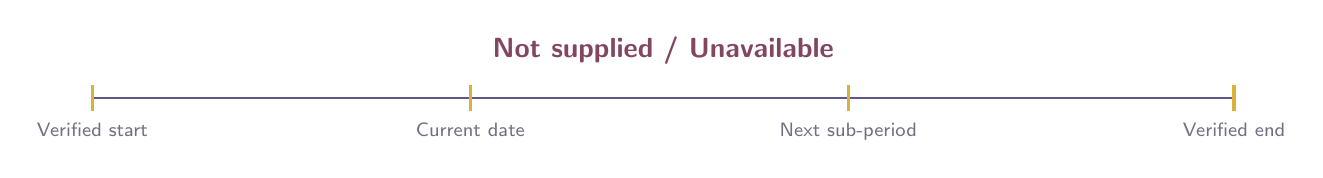
\begin{tikzpicture}[x=1cm,y=1cm]
  \draw[Purple,line width=1pt] (0,0)--(14.5,0);
  \foreach \x/\lab in {0/Verified start,4.8/Current date,9.6/Next sub-period,14.5/Verified end}{
    \draw[Gold,line width=1.2pt] (\x,-.16)--(\x,.16);
    \node[below=2mm,text=Muted,font=\sffamily\scriptsize,align=center] at (\x,0) {\lab};
  }
  \node[above=3mm,text=Burgundy,font=\sffamily\bfseries] at (7.25,0)
    {\CurrentAntardasha{} / \UpcomingPeriodLabel};
\end{tikzpicture}
\end{center}

\TwoCol{%
\begin{insightbox}
\BoxTitle{Opportunity language}
Identify the kind of responsibility, learning, visibility, network or transition that
may be more relevant—then state the practical preparation it deserves.
\end{insightbox}
}{%
\begin{goldbox}
\BoxTitle{Challenge language}
Describe the need for patience, review, boundaries, skill-building or financial
buffer. Avoid fear-based claims or event certainty.
\end{goldbox}
}

\begin{insightbox}
\BoxTitle{Upcoming periods and relevant career themes}
\UpcomingPeriods\par
\RelevantCareerThemes
\end{insightbox}

\ReportPage{TIMELINE}{Career Timeline}
{The final timeline will distinguish present context, upcoming emphasis and long-term development.}

\begin{center}

\begin{tikzpicture}[x=1cm,y=1cm]
  \fill[PalePurple,rounded corners=1mm] (0,0) rectangle (4.55,1.35);
  \fill[PaleGold,rounded corners=1mm] (4.85,0) rectangle (9.4,1.35);
  \fill[Mist,rounded corners=1mm] (9.7,0) rectangle (14.25,1.35);
  \node[font=\sffamily\bfseries,text=Navy] at (2.27,.88) {CURRENT PERIOD};
  \node[font=\sffamily\scriptsize,text=Burgundy] at (2.27,.43) {\CurrentPeriodLabel};
  \node[font=\sffamily\bfseries,text=Navy] at (7.12,.88) {UPCOMING PERIOD};
  \node[font=\sffamily\scriptsize,text=Burgundy] at (7.12,.43) {\UpcomingPeriodLabel};
  \node[font=\sffamily\bfseries,text=Navy] at (11.97,.88) {LONG-TERM PERIOD};
  \node[font=\sffamily\scriptsize,text=Burgundy] at (11.97,.43) {\LongTermPeriodLabel};
\end{tikzpicture}
\end{center}

{\small
\begin{tabularx}{\linewidth}{>{\sffamily\bfseries\color{Navy}}p{31mm} X X X}
\toprule
Period & Career theme & Potential opportunity & Recommended approach\\
\midrule
Current & \CurrentPeriodTheme & \CurrentPeriodOpportunity & \CurrentPeriodApproach\\
Upcoming & \UpcomingPeriodTheme & \UpcomingPeriodOpportunity & \UpcomingPeriodApproach\\
Long term & \LongTermPeriodTheme & \LongTermPeriodOpportunity & \LongTermPeriodApproach\\
\bottomrule
\end{tabularx}}

\vspace{4mm}
\begin{goldbox}
\BoxTitle{Production requirement}
Every important period should show exact dates, the relevant Dasha lords, the natal
reason the period matters, likely opportunities and challenges, and a practical
response. Transit overlays should use a stated reference date.
\end{goldbox}

\ReportPage{TIMING WINDOWS}{Major Opportunity Windows and Periods Requiring Patience}
{Timing is most useful when it changes preparation, pacing or the size of a commitment.}

\TwoCol{%
\begin{insightbox}
\BoxTitle{Opportunity window}
A supportive period may favor applications, visibility, responsibility, study,
networking, relocation exploration or business testing. The final report should name
the theme and the preparation—not promise an event.
\end{insightbox}
}{%
\begin{goldbox}
\BoxTitle{Patience period}
A demanding period may call for consolidation, proof-building, careful contracts,
lower leverage, stronger routines or delayed expansion. Patience is an active
strategy, not passive waiting.
\end{goldbox}
}

\begin{unavailablebox}
\BoxTitle{Opportunity and consolidation periods \hfill \DashaStatus}
\textbf{Opportunity periods:} \OpportunityPeriods\par
\textbf{Patience / consolidation periods:} \PatiencePeriods
\end{unavailablebox}

\begin{navybox}
\WhiteTitle{Decision use}
Timing should adjust \emph{how} the client proceeds: explore versus commit, prepare
versus launch, negotiate versus exit, diversify versus concentrate. It should not
remove the need for evidence and consent.
\end{navybox}

\ReportPage{OUTLOOK}{Career Transition Indicators and Short-Term Outlook}
{Transitions are assessed through repeated natal themes, active periods and real-world signals—not one transit in isolation.}

\TwoCol{%
\begin{insightbox}
\BoxTitle{Transition indicators}
Possible signals include activation of the 10th lord, links between the 6th/10th/11th
and change houses, nodal emphasis, or periods of planets strongly tied to professional
identity. Exact interpretation requires the chart.
\end{insightbox}
}{%
\begin{goldbox}
\BoxTitle{Short-term horizon}
The final report should define the horizon with dates, identify the dominant theme,
state what is and is not supported, and recommend one preparation step and one risk
control.
\end{goldbox}
}

\begin{unavailablebox}
\BoxTitle{Short-term outlook \hfill \DashaStatus}
\textbf{Transition indicators:} \CareerTransitionIndicators\par
\ShortTermOutlook
\end{unavailablebox}

\begin{navybox}
\WhiteTitle{Real-world confirmation}
Before acting, look for objective signals: changing mandate, sponsor support, market
demand, interview traction, financial runway, workload trend and family readiness.
\end{navybox}

\ReportPage{OUTLOOK}{Medium- and Long-Term Career Outlook}
{Long-range interpretation should emphasize development arcs rather than event-level certainty.}

\TwoCol{%
\begin{insightbox}
\BoxTitle{Medium term}
Usually framed around the next meaningful sub-periods: build capability, expand
responsibility, reposition, consolidate or prepare a transition. Exact dates and
planetary rationale belong in the final chart-based edition.
\end{insightbox}
}{%
\begin{goldbox}
\BoxTitle{Long term}
Focus on durable themes: the kind of authority built, how expertise compounds, the
role of institutions or independence, and how work evolves with maturity.
\end{goldbox}
}

\begin{navybox}
\WhiteTitle{Developmental lens}
Saturn may describe maturation through responsibility; Jupiter through knowledge and
judgment; the Sun through coherent authority; Mercury through adaptive competence;
the nodes through changing appetite and unfamiliar terrain. Placement and timing
decide which arc is relevant.
\end{navybox}

\begin{unavailablebox}
\BoxTitle{Client outlook \hfill \DashaStatus}
\textbf{Medium term:} \MediumTermOutlook\par
\textbf{Long term:} \LongTermOutlook
\end{unavailablebox}

% --------------------------------------------------------------------------
% PRACTICAL GUIDANCE
% --------------------------------------------------------------------------
\ReportPage{RECOMMENDATIONS}{Practical Career Recommendations}
{Astrological reflection becomes valuable when it produces a proportionate experiment, conversation or decision.}

\begin{insightbox}
\BoxTitle{Generated recommendations \hfill \ChartStatus}
\Recommendations
\end{insightbox}

\begin{navybox}
\WhiteTitle{Universal recommendations for the current data stage}
\begin{enumerate}
  \item Verify the birth record and calculation configuration before personalization.
  \item Define the current decision in one sentence: role, field, work mode, location,
  timing or development priority.
  \item Gather factual evidence: performance feedback, skill proof, finances, market
  demand, constraints and stakeholder views.
  \item Use the chart-based report to generate hypotheses and counter-hypotheses.
  \item Test the preferred direction with the smallest credible real-world experiment.
\end{enumerate}
\end{navybox}

\vspace{3mm}
\TwoCol{%
\begin{insightbox}
\BoxTitle{A good experiment}
Has a clear question, limited downside, observable result and review date. Examples
include a scoped project, informational interview, client pilot or portfolio case.
\end{insightbox}
}{%
\begin{goldbox}
\BoxTitle{A poor experiment}
Requires irreversible commitment before basic evidence, relies on one prediction, or
confuses urgency with readiness.
\end{goldbox}
}

\ReportPage{DEVELOPMENT}{Professional Priorities, Skills and Mistakes to Avoid}
{The final development plan should focus on the few capabilities that unlock the chart’s strongest career theme.}

{\small
\begin{tabularx}{\linewidth}{>{\sffamily\bfseries\color{Navy}}p{36mm} X X}
\toprule
Area & Production-report output & Client-specific priority\\
\midrule
Professional priority & One primary, one supporting & \PrimaryProfessionalPriority\\
Technical skill & Specific capability and proof & \TechnicalSkillPriority\\
Communication skill & Audience, medium and standard & \CommunicationSkillPriority\\
Leadership skill & Behavior under responsibility & \LeadershipSkillPriority\\
Network skill & Relationship category and cadence & \NetworkSkillPriority\\
Mistake to avoid & Trigger, behavior, countermeasure & \MistakeToAvoid\\
\bottomrule
\end{tabularx}}

\vspace{4mm}
\begin{navybox}
\WhiteTitle{Development rule}
Choose skills that are both chart-consistent and market-relevant. A symbolic strength
without practiced competence is potential; a market trend without personal fit may
be difficult to sustain.
\end{navybox}

\begin{goldbox}
\BoxTitle{Do not overcorrect}
A challenge should not become an identity project. Select one behavior, one context
and one feedback mechanism; review progress before adding another intervention.
\end{goldbox}

\begin{unavailablebox}
\BoxTitle{Generated development priorities \hfill \ChartStatus}
\ProfessionalDevelopmentPriorities
\end{unavailablebox}

\ReportPage{DECISIONS}{Career Decision Framework}
{Use the report to improve a real decision—not to outsource the decision.}

\begin{center}
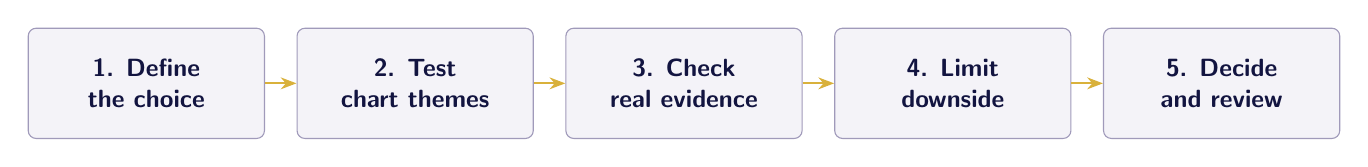
\begin{tikzpicture}[node distance=4mm]
  \tikzset{d/.style={draw=Purple!60,fill=Mist,rounded corners=1mm,minimum width=30mm,
    minimum height=14mm,align=center,font=\sffamily\small\bfseries,text=Navy},
    a/.style={-{Stealth[length=2mm]},Gold,line width=.8pt}}
  \node[d] (a) {1. Define\\the choice};
  \node[d,right=of a] (b) {2. Test\\chart themes};
  \node[d,right=of b] (c) {3. Check\\real evidence};
  \node[d,right=of c] (d) {4. Limit\\downside};
  \node[d,right=of d] (e) {5. Decide\\and review};
  \draw[a] (a)--(b);\draw[a] (b)--(c);\draw[a] (c)--(d);\draw[a] (d)--(e);
\end{tikzpicture}
\end{center}

\begin{enumerate}
  \item \textbf{Define the choice.} State the options, deadline and non-negotiables.
  \item \textbf{Test chart themes.} Record supportive and contradictory factors.
  \item \textbf{Check real evidence.} Skills, opportunity quality, people, finances,
  health, ethics and constraints.
  \item \textbf{Limit downside.} Pilot, stage, negotiate, insure or preserve runway.
  \item \textbf{Decide and review.} Choose based on the combined case; set a review date.
\end{enumerate}

\begin{goldbox}
\BoxTitle{Decision principle}
The right use of astrology is reflective: it may reveal a pattern or timing theme that
deserves attention. The final choice remains the client’s.
\end{goldbox}

\begin{insightbox}
\BoxTitle{Client decision guidance \hfill \ChartStatus}
\DecisionGuidance
\end{insightbox}

\ReportPage{ACTION PLAN}{30-Day, 90-Day, 1-Year and 3-Year Direction}
{A staged plan turns insight into evidence while preserving room to learn.}

{\small
\begin{tabularx}{\linewidth}{>{\sffamily\bfseries\color{Navy}}p{25mm} X X}
\toprule
Horizon & Focus & Generated action\\
\midrule
30 days & Clarity and verification &
\ThirtyDayFocus\\
90 days & Evidence and relationships &
\NinetyDayFocus\\
1 year & Position and responsibility &
\OneYearFocus\\
3 years & Direction and leverage &
\ThreeYearDirection\\
\bottomrule
\end{tabularx}}

\vspace{4mm}
\begin{unavailablebox}
\BoxTitle{Personalization boundary \hfill \ChartStatus}
\ActionPlanSummary
\end{unavailablebox}

\ReportPage{FINAL SYNTHESIS}{Final Career Summary}
{The finished report will close with one coherent view of strengths, environment, direction, timing and agency.}

\begin{navybox}
\WhiteTitle{Final generated synthesis}
This document demonstrates a disciplined consultation architecture: career identity
is anchored in the Ascendant and 10th house; work, income and gains are tested through
the 6th, 2nd and 11th; intelligence, learning and global context are added through the
5th, 9th and 12th; each planet is interpreted by actual placement; and timing is
withheld unless dates are verified.
\end{navybox}

\vspace{3mm}
\begin{unavailablebox}
\BoxTitle{Client-specific conclusion \hfill \ChartStatus}
\FinalSynthesis
\end{unavailablebox}

\vspace{3mm}
\begin{goldbox}
\BoxTitle{Next production step}
Supply the exact Astro Sushil logo asset and a verified generated
\texttt{report\_data.tex}. The rendering template will then display evidence-linked
interpretation while preserving the cautious language and practical decision structure.
\end{goldbox}

\ReportPage{CLOSING}{Your Career, Your Choices}
{Astrology may offer a language for pattern and timing. Direction is shaped through attention, practice and choice.}

\vspace{5mm}
\begin{center}
{\displayfont\fontsize{26}{31}\selectfont\color{Navy}
Your Career,\par Your Choices\par}
\vspace{5mm}
{\color{Gold}\rule{46mm}{1pt}}\par
\vspace{6mm}
\begin{minipage}{0.72\linewidth}
\centering
\fontsize{12}{17}\selectfont\color{Purple}
Build expertise that compounds. Choose environments that support clear judgment.
Treat timing as context, not command. Test important decisions against evidence,
values and the life you want to sustain.
\end{minipage}
\vspace{14mm}

\BrandLight[48mm]\par
\vspace{4mm}
{\sffamily\fontsize{10}{14}\selectfont\color{Burgundy}
Explore your chart. Understand yourself. Make informed choices.}
\vfill
{\sffamily\fontsize{8}{10}\selectfont\color{Muted}
© 2026 Astro Sushil. All rights reserved.}
\end{center}

\ReportPage{METHODOLOGY}{Methodology, Disclaimer and Confidentiality}
{The final page states the interpretive limits, data basis and client privacy standard without ambiguity.}

\begin{insightbox}
\BoxTitle{Methodology}
The intended production report uses traditional Vedic astrology, the verified birth
record and the exact calculation settings supplied by Astro Sushil. It synthesizes
the natal chart, career-relevant houses and lords, planetary condition, verified
yogas, and Vimshottari Dasha or transit information when available.
\MethodologyDataNote
\end{insightbox}

\begin{unavailablebox}
\BoxTitle{Disclaimer}
This report is an interpretive reading based on traditional Vedic astrology
principles and the birth information supplied for this report. Astrology is not a
scientifically established method for predicting future events. The interpretations
provided should be treated as guidance and reflection rather than certainty. This
report should not replace qualified professional advice regarding medical, financial,
legal, career, or other high-stakes decisions.
\end{unavailablebox}

\begin{goldbox}
\BoxTitle{Confidentiality}
This report format is marked \textbf{CONFIDENTIAL PERSONAL REPORT}. A completed report
may contain personally identifying birth information and should be treated as private.
Share it only with the client’s consent and store source data appropriately.
\end{goldbox}

\vfill
\begin{center}
\BrandLight[45mm]\par
\vspace{3mm}
{\sffamily\fontsize{8}{10}\selectfont\color{Muted}
© 2026 Astro Sushil. All rights reserved.}
\end{center}

\end{document}
